%&preformat-disser
\RequirePackage[l2tabu,orthodox]{nag} % Раскомментировав, можно в логе получать рекомендации относительно правильного использования пакетов и предупреждения об устаревших и нерекомендуемых пакетах
% Формат А4, 14pt (ГОСТ Р 7.0.11-2011, 5.3.6)
\documentclass[a4paper,14pt,oneside,openany]{memoir}

\input{common/setup}               % общие настройки шаблона
\input{common/packages}  % Пакеты общие для диссертации и автореферата
\input{Dissertation/dispackages}         % Пакеты для диссертации
\usepackage{tabu, tabulary}  %таблицы с автоматически подбирающейся шириной столбцов
\usepackage{fr-longtable}    %ради \endlasthead

% Листинги с исходным кодом программ
\usepackage{fancyvrb}
\usepackage{listings}
\usepackage[linesnumbered,boxed]{algorithm2e}

% Русская традиция начертания греческих букв
%\usepackage{upgreek} % прямые греческие ради русской традиции

% Микротипографика
%\ifnumequal{\value{draft}}{0}{% Только если у нас режим чистовика
%    \usepackage[final]{microtype}[2016/05/14] % улучшает представление букв и слов в строках, может помочь при наличии отдельно висящих слов
%}{}

% Отметка о версии черновика на каждой странице
% Чтобы работало надо в своей локальной копии по инструкции
% https://www.ctan.org/pkg/gitinfo2 создать небходимые файлы в папке
% ./git/hooks
% If you’re familiar with tweaking git, you can probably work it out for
% yourself. If not, I suggest you follow these steps:
% 1. First, you need a git repository and working tree. For this example,
% let’s suppose that the root of the working tree is in ~/compsci
% 2. Copy the file post-xxx-sample.txt (which is in the same folder of
% your TEX distribution as this pdf) into the git hooks directory in your
% working copy. In our example case, you should end up with a file called
% ~/compsci/.git/hooks/post-checkout
% 3. If you’re using a unix-like system, don’t forget to make the file executable.
% Just how you do this is outside the scope of this manual, but one
% possible way is with commands such as this:
% chmod g+x post-checkout.
% 4. Test your setup with “git checkout master” (or another suitable branch
% name). This should generate copies of gitHeadInfo.gin in the directories
% you intended.
% 5. Now make two more copies of this file in the same directory (hooks),
% calling them post-commit and post-merge, and you’re done. As before,
% users of unix-like systems should ensure these files are marked as
% executable.
\ifnumequal{\value{draft}}{1}{% Черновик
   \IfFileExists{.git/gitHeadInfo.gin}{                                        
      \usepackage[mark,pcount]{gitinfo2}
      \renewcommand{\gitMark}{rev.\gitAbbrevHash\quad\gitCommitterEmail\quad\gitAuthorIsoDate}
      \renewcommand{\gitMarkFormat}{\color{Gray}\small\bfseries}
   }{}
}{}        % Пакеты для специфических пользовательских задач

\input{Dissertation/setup}               % Упрощённые настройки шаблона

\input{Dissertation/preamblenames}       % Переопределение именований, чтобы можно было и в преамбуле использовать
% Новые переменные, которые могут использоваться во всём проекте
% ГОСТ 7.0.11-2011
% 9.2 Оформление текста автореферата диссертации
% 9.2.1 Общая характеристика работы включает в себя следующие основные структурные
% элементы:
% актуальность темы исследования;
\newcommand{\actualityTXT}{Актуальность темы.}
% степень ее разработанности;
\newcommand{\progressTXT}{Степень разработанности темы.}
% цели и задачи;
\newcommand{\aimTXT}{Целью}
\newcommand{\tasksTXT}{задачи}
% научную новизну;
\newcommand{\noveltyTXT}{Научная новизна:}
% теоретическую и практическую значимость работы;
%\newcommand{\influenceTXT}{Теоретическая и практическая значимость}
% или чаще используют просто
\newcommand{\influenceTXT}{Практическая значимость}
% методологию и методы исследования;
\newcommand{\methodsTXT}{Mетодология и методы исследования.}
% положения, выносимые на защиту;
\newcommand{\defpositionsTXT}{Основные положения, выносимые на~защиту:}
% степень достоверности и апробацию результатов.
\newcommand{\reliabilityTXT}{Достоверность}
\newcommand{\probationTXT}{Апробация работы.}

\newcommand{\contributionTXT}{Личный вклад.}
\newcommand{\publicationsTXT}{Публикации.}


\newcommand{\authorbibtitle}{Публикации автора по теме диссертации}
\newcommand{\fullbibtitle}{Список литературы} % (ГОСТ Р 7.0.11-2011, 4)

\DeclareMathOperator*{\argmin}{arg\,min}
\DeclareMathOperator*{\argmax}{arg\,max}

\newcommand{\vakbibtitle}{В изданиях из списка ВАК РФ}
\newcommand{\notvakbibtitle}{В прочих изданиях}
\newcommand{\confbibtitle}{В сборниках трудов конференций}  % Новые переменные, которые могут использоваться во всём проекте

%%% Основные сведения %%%
\newcommand{\thesisAuthor}             % Диссертация, ФИО автора
{%
    \texorpdfstring{% \texorpdfstring takes two arguments and uses the first for (La)TeX and the second for pdf
        Шальнов Евгений Вадимович% так будет отображаться на титульном листе или в тексте, где будет использоваться переменная
    }{%
        Шальнов, Евгений Вадимович% эта запись для свойств pdf-файла. В таком виде, если pdf будет обработан программами для сбора библиографических сведений, будет правильно представлена фамилия.
    }%
}
\newcommand{\thesisAuthorShort}        % Диссертация, ФИО автора инициалами
{Е.В.~Шальнов}

\newcommand{\thesisUdk}                % Диссертация, УДК
{\todo{xxx.xxx}}
\newcommand{\thesisTitle}              % Диссертация, название
{\texorpdfstring{\MakeUppercase{Порождающий подхок к выделению и сопровождению объектов в видео}}{Название диссертационной работы}}
\newcommand{\thesisSpecialtyNumber}    % Диссертация, специальность, номер
{\texorpdfstring{05.13.11}{05.13.11}}
\newcommand{\thesisSpecialtyTitle}     % Диссертация, специальность, название
{\texorpdfstring{Математическое и программное обеспечение вычислительных машин, комплексов и компьютерных сетей}{Название специальности}}
\newcommand{\thesisDegree}             % Диссертация, ученая степень
{кандидата физико-математических наук}
\newcommand{\thesisDegreeShort}        % Диссертация, ученая степень, краткая запись
{канд. физ.-мат. наук}
\newcommand{\thesisCity}               % Диссертация, город защиты
{Москва}
\newcommand{\thesisYear}               % Диссертация, год защиты
{2017}
\newcommand{\thesisOrganization}       % Диссертация, организация
{Московский Государственный Университет имени М.В.~Ломоносова}
\newcommand{\thesisOrganizationShort}  % Диссертация, краткое название организации для доклада
{МГУ имени М.В.~Ломоносова}

\newcommand{\thesisInOrganization}     % Диссертация, организация в предложном падеже: Работа выполнена в ...
{Московском Государственном Университете имени М.В.~Ломоносова}

\newcommand{\supervisorFio}            % Научный руководитель, ФИО
{Конушин Антон Сергеевич}
\newcommand{\supervisorRegalia}        % Научный руководитель, регалии
{кандидат физико-математических наук, доцент}
\newcommand{\supervisorFioShort}       % Научный руководитель, ФИО
{А.С.~Конушин}
\newcommand{\supervisorRegaliaShort}   % Научный руководитель, регалии
{канд.~физ.-мат.~наук,~доц.}


\newcommand{\opponentOneFio}           % Оппонент 1, ФИО
{\todo{Фамилия Имя Отчество}}
\newcommand{\opponentOneRegalia}       % Оппонент 1, регалии
{\todo{доктор физико-математических наук, профессор}}
\newcommand{\opponentOneJobPlace}      % Оппонент 1, место работы
{\todo{Не очень длинное название для места работы}}
\newcommand{\opponentOneJobPost}       % Оппонент 1, должность
{\todo{старший научный сотрудник}}

\newcommand{\opponentTwoFio}           % Оппонент 2, ФИО
{\todo{Фамилия Имя Отчество}}
\newcommand{\opponentTwoRegalia}       % Оппонент 2, регалии
{\todo{кандидат физико-математических наук}}
\newcommand{\opponentTwoJobPlace}      % Оппонент 2, место работы
{\todo{Основное место работы c длинным длинным длинным длинным названием}}
\newcommand{\opponentTwoJobPost}       % Оппонент 2, должность
{\todo{старший научный сотрудник}}

\newcommand{\leadingOrganizationTitle} % Ведущая организация, дополнительные строки
{\todo{Федеральное государственное бюджетное образовательное учреждение высшего профессионального образования с~длинным длинным длинным длинным названием}}

\newcommand{\defenseDate}              % Защита, дата
{\todo{DD mmmmmmmm YYYY~г.~в~XX часов}}
\newcommand{\defenseCouncilNumber}     % Защита, номер диссертационного совета
{\todo{Д\,123.456.78}}
\newcommand{\defenseCouncilTitle}      % Защита, учреждение диссертационного совета
{\todo{Название учреждения}}
\newcommand{\defenseCouncilAddress}    % Защита, адрес учреждение диссертационного совета
{\todo{Адрес}}
\newcommand{\defenseCouncilPhone}      % Телефон для справок
{\todo{+7~(0000)~00-00-00}}

\newcommand{\defenseSecretaryFio}      % Секретарь диссертационного совета, ФИО
{\todo{Фамилия Имя Отчество}}
\newcommand{\defenseSecretaryRegalia}  % Секретарь диссертационного совета, регалии
{\todo{д-р~физ.-мат. наук}}            % Для сокращений есть ГОСТы, например: ГОСТ Р 7.0.12-2011 + http://base.garant.ru/179724/#block_30000

\newcommand{\synopsisLibrary}          % Автореферат, название библиотеки
{\todo{Название библиотеки}}
\newcommand{\synopsisDate}             % Автореферат, дата рассылки
{\todo{DD mmmmmmmm YYYY года}}

% To avoid conflict with beamer class use \providecommand
\providecommand{\keywords}%            % Ключевые слова для метаданных PDF диссертации и автореферата
{}      % Основные сведения
\input{common/styles}    % Стили общие для диссертации и автореферата
%%% Изображения %%%
\graphicspath{{images/}{Dissertation/images/}}         % Пути к изображениям

%%% Макет страницы %%%
% Выставляем значения полей (ГОСТ 7.0.11-2011, 5.3.7)
\geometry{a4paper,top=2cm,bottom=2cm,left=2.5cm,right=1cm,nofoot,nomarginpar} %,showframe
\setlength{\topskip}{0pt}   %размер дополнительного верхнего поля

%%% Интервалы %%%
%% По ГОСТ Р 7.0.11-2011, пункту 5.3.6 требуется полуторный интервал
%% Реализация средствами класса (на основе setspace) ближе к типографской классике.
%% И правит сразу и в таблицах (если со звёздочкой) 
%\DoubleSpacing*     % Двойной интервал
\OnehalfSpacing*    % Полуторный интервал
\setSpacing{1.42}   % Полуторный интервал, подобный Ворду (возможно, стоит включать вместе с предыдущей строкой)

%%% Выравнивание и переносы %%%
%% http://tex.stackexchange.com/questions/241343/what-is-the-meaning-of-fussy-sloppy-emergencystretch-tolerance-hbadness
%% http://www.latex-community.org/forum/viewtopic.php?p=70342#p70342
\tolerance 1414
\hbadness 1414
\emergencystretch 1.5em % В случае проблем регулировать в первую очередь
\hfuzz 0.3pt
\vfuzz \hfuzz
%\raggedbottom
%\sloppy                 % Избавляемся от переполнений
\clubpenalty=10000      % Запрещаем разрыв страницы после первой строки абзаца
\widowpenalty=10000     % Запрещаем разрыв страницы после последней строки абзаца

%%% Блок управления параметрами для выравнивания заголовков в тексте %%%
\newlength{\otstuplen}
\setlength{\otstuplen}{\theotstup\parindent}
\ifnumequal{\value{headingalign}}{0}{% выравнивание заголовков в тексте
    \newcommand{\hdngalign}{\centering}                % по центру
    \newcommand{\hdngaligni}{}% по центру
    \setlength{\otstuplen}{0pt}
}{%
    \newcommand{\hdngalign}{}                 % по левому краю
    \newcommand{\hdngaligni}{\hspace{\otstuplen}}      % по левому краю
} % В обоих случаях вроде бы без переноса, как и надо (ГОСТ Р 7.0.11-2011, 5.3.5)

%%% Оглавление %%%
\renewcommand{\cftchapterdotsep}{\cftdotsep}                % отбивка точками до номера страницы начала главы/раздела

%% Переносить слова в заголовке не допускается (ГОСТ Р 7.0.11-2011, 5.3.5). Заголовки в оглавлении должны точно повторять заголовки в тексте (ГОСТ Р 7.0.11-2011, 5.2.3). Прямого указания на запрет переносов в оглавлении нет, но по той же логике невнесения искажений в смысл, лучше в оглавлении не переносить:
\setrmarg{2.55em plus1fil}                             %To have the (sectional) titles in the ToC, etc., typeset ragged right with no hyphenation
\renewcommand{\cftchapterpagefont}{\normalfont}        % нежирные номера страниц у глав в оглавлении
\renewcommand{\cftchapterleader}{\cftdotfill{\cftchapterdotsep}}% нежирные точки до номеров страниц у глав в оглавлении
%\renewcommand{\cftchapterfont}{}                       % нежирные названия глав в оглавлении

\ifnumgreater{\value{headingdelim}}{0}{%
    \renewcommand\cftchapteraftersnum{.\space}       % добавляет точку с пробелом после номера раздела в оглавлении
}{}
\ifnumgreater{\value{headingdelim}}{1}{%
    \renewcommand\cftsectionaftersnum{.\space}       % добавляет точку с пробелом после номера подраздела в оглавлении
    \renewcommand\cftsubsectionaftersnum{.\space}    % добавляет точку с пробелом после номера подподраздела в оглавлении
    \renewcommand\cftsubsubsectionaftersnum{.\space} % добавляет точку с пробелом после номера подподподраздела в оглавлении
    \AtBeginDocument{% без этого polyglossia сама всё переопределяет
        \setsecnumformat{\csname the#1\endcsname.\space}
    }
}{%
    \AtBeginDocument{% без этого polyglossia сама всё переопределяет
        \setsecnumformat{\csname the#1\endcsname\quad}
    }
}

\ifnumequal{\value{pgnum}}{1}{%
    \addtocontents{toc}{~\hfill{Стр.}\par}% добавить Стр. над номерами страниц
}{}

\renewcommand*{\cftappendixname}{\appendixname\space} % Слово Приложение в оглавлении

%%% Колонтитулы %%%
% Порядковый номер страницы печатают на середине верхнего поля страницы (ГОСТ Р 7.0.11-2011, 5.3.8)
\makeevenhead{plain}{}{\thepage}{}
\makeoddhead{plain}{}{\thepage}{}
\makeevenfoot{plain}{}{}{}
\makeoddfoot{plain}{}{}{}
\pagestyle{plain}

%%% Оформление заголовков глав, разделов, подразделов %%%
%% Работа должна быть выполнена ... размером шрифта 12-14 пунктов (ГОСТ Р 7.0.11-2011, 5.3.8). То есть не должно быть надписей шрифтом более 14. Так и поставим.
%% Эти установки будут давать одинаковый результат независимо от выбора базовым шрифтом 12 пт или 14 пт
\newcommand{\basegostsectionfont}{\fontsize{14pt}{16pt}\selectfont\bfseries}

\makechapterstyle{thesisgost}{%
    \chapterstyle{default}
    \setlength{\beforechapskip}{0pt}
    \setlength{\midchapskip}{0pt}
    \setlength{\afterchapskip}{\theintvl\curtextsize}
    \renewcommand*{\chapnamefont}{\basegostsectionfont}
    \renewcommand*{\chapnumfont}{\basegostsectionfont}
    \renewcommand*{\chaptitlefont}{\basegostsectionfont}
    \renewcommand*{\chapterheadstart}{}
    \ifnumgreater{\value{headingdelim}}{0}{%
        \renewcommand*{\afterchapternum}{.\space}   % добавляет точку с пробелом после номера раздела
    }{%
        \renewcommand*{\afterchapternum}{\quad}     % добавляет \quad после номера раздела
    }
    \renewcommand*{\printchapternum}{\hdngaligni\hdngalign\chapnumfont \thechapter}
    \renewcommand*{\printchaptername}{}
    \renewcommand*{\printchapternonum}{\hdngaligni\hdngalign}
}

\makeatletter
\makechapterstyle{thesisgostchapname}{%
    \chapterstyle{thesisgost}
    \renewcommand*{\printchapternum}{\chapnumfont \thechapter}
    \renewcommand*{\printchaptername}{\hdngaligni\hdngalign\chapnamefont \@chapapp} %
}
\makeatother

\chapterstyle{thesisgost}

\setsecheadstyle{\basegostsectionfont\hdngalign}
\setsecindent{\otstuplen}

\setsubsecheadstyle{\basegostsectionfont\hdngalign}
\setsubsecindent{\otstuplen}

\setsubsubsecheadstyle{\basegostsectionfont\hdngalign}
\setsubsubsecindent{\otstuplen}

\sethangfrom{\noindent #1} %все заголовки подразделов центрируются с учетом номера, как block 

\ifnumequal{\value{chapstyle}}{1}{%
    \chapterstyle{thesisgostchapname}
    \renewcommand*{\cftchaptername}{\chaptername\space} % будет вписано слово Глава перед каждым номером раздела в оглавлении
}{}%

%%% Интервалы между заголовками
\setbeforesecskip{\theintvl\curtextsize}% Заголовки отделяют от текста сверху и снизу тремя интервалами (ГОСТ Р 7.0.11-2011, 5.3.5).
\setaftersecskip{\theintvl\curtextsize}
\setbeforesubsecskip{\theintvl\curtextsize}
\setaftersubsecskip{\theintvl\curtextsize}
\setbeforesubsubsecskip{\theintvl\curtextsize}
\setaftersubsubsecskip{\theintvl\curtextsize}

%%% Блок дополнительного управления размерами заголовков
\ifnumequal{\value{headingsize}}{1}{% Пропорциональные заголовки и базовый шрифт 14 пт
    \renewcommand{\basegostsectionfont}{\large\bfseries}
    \renewcommand*{\chapnamefont}{\Large\bfseries}
    \renewcommand*{\chapnumfont}{\Large\bfseries}
    \renewcommand*{\chaptitlefont}{\Large\bfseries}
}{}

%%% Счётчики %%%

%% Упрощённые настройки шаблона диссертации: нумерация формул, таблиц, рисунков
\ifnumequal{\value{contnumeq}}{1}{%
    \counterwithout{equation}{chapter} % Убираем связанность номера формулы с номером главы/раздела
}{}
\ifnumequal{\value{contnumfig}}{1}{%
    \counterwithout{figure}{chapter}   % Убираем связанность номера рисунка с номером главы/раздела
}{}
\ifnumequal{\value{contnumtab}}{1}{%
    \counterwithout{table}{chapter}    % Убираем связанность номера таблицы с номером главы/раздела
}{}


%%http://www.linux.org.ru/forum/general/6993203#comment-6994589 (используется totcount)
\makeatletter
\def\formbytotal#1#2#3#4#5{%
    \newcount\@c
    \@c\totvalue{#1}\relax
    \newcount\@last
    \newcount\@pnul
    \@last\@c\relax
    \divide\@last 10
    \@pnul\@last\relax
    \divide\@pnul 10
    \multiply\@pnul-10
    \advance\@pnul\@last
    \multiply\@last-10
    \advance\@last\@c
    \total{#1}~#2%
    \ifnum\@pnul=1#5\else%
    \ifcase\@last#5\or#3\or#4\or#4\or#4\else#5\fi
    \fi
}
\makeatother

\AtBeginDocument{
%% регистрируем счётчики в системе totcounter
    \regtotcounter{totalcount@figure}
    \regtotcounter{totalcount@table}       % Если иным способом поставить в преамбуле то ошибка в числе таблиц
    \regtotcounter{TotPages}               % Если иным способом поставить в преамбуле то ошибка в числе страниц
}

%%% Правильная нумерация приложений %%%
%% По ГОСТ 2.105, п. 4.3.8 Приложения обозначают заглавными буквами русского алфавита,
%% начиная с А, за исключением букв Ё, З, Й, О, Ч, Ь, Ы, Ъ.
%% Здесь также переделаны все нумерации русскими буквами.
\ifxetexorluatex
    \makeatletter
    \def\russian@Alph#1{\ifcase#1\or
       А\or Б\or В\or Г\or Д\or Е\or Ж\or
       И\or К\or Л\or М\or Н\or
       П\or Р\or С\or Т\or У\or Ф\or Х\or
       Ц\or Ш\or Щ\or Э\or Ю\or Я\else\xpg@ill@value{#1}{russian@Alph}\fi}
    \def\russian@alph#1{\ifcase#1\or
       а\or б\or в\or г\or д\or е\or ж\or
       и\or к\or л\or м\or н\or
       п\or р\or с\or т\or у\or ф\or х\or
       ц\or ш\or щ\or э\or ю\or я\else\xpg@ill@value{#1}{russian@alph}\fi}
    \makeatother
\else
    \makeatletter
    \if@uni@ode
      \def\russian@Alph#1{\ifcase#1\or
        А\or Б\or В\or Г\or Д\or Е\or Ж\or
        И\or К\or Л\or М\or Н\or
        П\or Р\or С\or Т\or У\or Ф\or Х\or
        Ц\or Ш\or Щ\or Э\or Ю\or Я\else\@ctrerr\fi}
    \else
      \def\russian@Alph#1{\ifcase#1\or
        \CYRA\or\CYRB\or\CYRV\or\CYRG\or\CYRD\or\CYRE\or\CYRZH\or
        \CYRI\or\CYRK\or\CYRL\or\CYRM\or\CYRN\or
        \CYRP\or\CYRR\or\CYRS\or\CYRT\or\CYRU\or\CYRF\or\CYRH\or
        \CYRC\or\CYRSH\or\CYRSHCH\or\CYREREV\or\CYRYU\or
        \CYRYA\else\@ctrerr\fi}
    \fi
    \if@uni@ode
      \def\russian@alph#1{\ifcase#1\or
        а\or б\or в\or г\or д\or е\or ж\or
        и\or к\or л\or м\or н\or
        п\or р\or с\or т\or у\or ф\or х\or
        ц\or ш\or щ\or э\or ю\or я\else\@ctrerr\fi}
    \else
      \def\russian@alph#1{\ifcase#1\or
        \cyra\or\cyrb\or\cyrv\or\cyrg\or\cyrd\or\cyre\or\cyrzh\or
        \cyri\or\cyrk\or\cyrl\or\cyrm\or\cyrn\or
        \cyrp\or\cyrr\or\cyrs\or\cyrt\or\cyru\or\cyrf\or\cyrh\or
        \cyrc\or\cyrsh\or\cyrshch\or\cyrerev\or\cyryu\or
        \cyrya\else\@ctrerr\fi}
    \fi
    \makeatother
\fi           % Стили для диссертации
\input{Dissertation/userstyles}          % Стили для специфических пользовательских задач
\input{biblio/bibliopreamble}% Настройки библиографии из внешнего файла (там же выбор: встроенная или на основе biblatex)

\input{Dissertation/inclusioncontrol}    % Управление компиляцией отдельных частей диссертации

\begin{document}

\input{common/renames}                   % Переопределение именований

% Структура диссертации (ГОСТ Р 7.0.11-2011, 4)
\include{Dissertation/title}           % Титульный лист
\include{Dissertation/contents}        % Оглавление
\include{Dissertation/introduction}    % Введение
% !TeX spellcheck = ru_RU
\chapter{Обзор литературы}  \label{chapt1}

\section{Определение позы камеры}

Задача автоматического определения позы камеры в сцене исследуется давно \cite{caprile1990using}, \cite{li2010simultaneous}, \cite{liu2011surveillance} ,\cite{chen2007accurate}, \cite{pflugfelder2007people}, \cite{den2015automatic}, \cite{puwein2012ptz}, \cite{dubska2014automatic}. Её решением является метод построения отображения мировой системы координат в систему координат, связанную с камерой.

Для решения этой задачи используется информация, извлекаемая из наблюдаемой видеопоследовательности. В работе \cite{puwein2012ptz} представлен подход, получающий информацию о камере при её движении. Авторы использовали сопровождение ключевых точек при повороте камеры и изменении масштаба. Это позволило оценить фокусное расстояние камеры и направление осей мировой системы координат. В то же время большое количество камер видеонаблюдения являются статичными, то есть не изменяют своего положения и направления в сцене с течением времению. В своей работе я рассматриваю только данные, в которых камера не изменяет свою позу, то есть камера неподвижна.

Я выделяю два подхода решения задачи определения позы камеры в случае неподвижной камеры. Алгоритмы первого подхода анализируют прямые на изображении сцены для восстановления мировой системы координат, в то время, как алгоритмы второго подхода анализируют размеры объектов на изображении.

\subsection{Анализ прямых на изображении}

Ключевым предположением методов первого подхода является наблюдение, так называемого, <<Манхэттенского мира>>, то есть сцены созданной человеком, где у наблюдаемых прямых преобладают три ортогональных направления: два горизонтальных и одно вертикальное. Авторы этих работ предлагают использовать направления этих прямых в качестве направлений базисных векторов мировой системы координат. Такой выбор обусловлен тем, что из-за структуры сцены в точках схода (ТС), соответствующих этим направлениям, пересекается наибольшее количество наблюдаемых прямых. Поэтому работы первого подхода направлены на локализацию этих точке схода на изображении. Для краткости в дальнейшем точки схода, соответствующие ортогональным прямым сцены, я буду называть ортогональными. В работе \cite{caprile1990using} представлено соотношение между положением трех ортогональных точек схода (ТОТС) и фокусным расстоянием камеры. Оно послужило основой для последующих алгоритмов определения позы камеры. В работе \cite{li2010simultaneous} предлагается извлекать ортогональные прямые из изображения объектов, таких как здания. Однако предложенный метод не может быть применен в сценах, где такие структуры отсутствуют, или не все необходимые ТС могут быть найдены. Поэтому в работе \cite{dubska2014automatic} предлагается использовать видимое направление движения автомобилей по автостраде для поиска горизонтальных ТС. В работах \cite{chen2007accurate}, \cite{liu2011surveillance}, \cite{den2015automatic} предлагается использовать направление движения людей и ориентацию их изображения для поиска линии горизонта и вертикальной ТС. Авторы используют информацию о росте людей для оценки положения камеры в сцене. В работе \cite{den2015automatic} предполагается, что рост всех людей одинаков и равен 1.8 метра, в то время как авторы \cite{liu2011surveillance} используют оцененное распределение роста европейцев \cite{visscher2008sizing}.В работах \cite{chen2007accurate}, \cite{liu2011surveillance} используется ориентация областей переднего плана, соответствующих людям, для определения вертикального направления на изображении. В описанных работах люди моделируются вертикальными отрезками. Точность такой модели существенно понижается, когда направление съемки камеры отличается от горизонтального.

\subsection{Анализ размеров объектов на изображении}

Алгоритмы второго подхода анализируют распределение размеров объектов на изображении сцены. Классическим предположением этих методов является наличие единственной плоскости земли, на которой располагаются все объекты. Самым известный алгоритм этого подхода был предложен в работе \cite{hoiem2008putting}. Авторы построили вероятностную графическую графическую модель, описывающую зависимость между положением камеры и размерами объектов в сцене. Предложенный алгоритм имеет ряд существенных недостатков. Одним из ключевых является предположение высокой точности исспользуемого детектора объектов. Также авторы предполагают, что направление съемки камеры близко к горизонтальному. Это позволило авторам построить аналитическую формулу отображения положения камеры в размер объекта на изображении.

В этой работе я предлагаю алгоритм относящийся ко второму подходу. В отличие от предыдущих методов предложенных алгоритм не зависит от направления съемки камеры и может быть адаптирован для любого алгоритма поиска объектов на изображении. В своей работе я предполагаю наличие ложных обнаружений среди результатов работы детектора.

\section{Локализация объектов}

Задача построения детектора объектов на изображении всегда интересовала исследователей в области компьютерного зрения. Обычно на разрабатываемые алгоритмы накладывали требования по времени работы и количеству ложных срабатываний. Эти ограничания зачастую противоречили друг другу. Действительно, часто повышение точности классификатора окон приводит к повышению его вычислительной сложности. Для практического применения в видеонаблюдении скорость обработки данных является ключевым параметром. Поэтому многие методы разрабатывали способы понижения вычислительной сложности детекторов при сохранении их качества. Можно выделить два основных направления работы в этой области: построение быстрого классификатора и уменьшение количества рассматриваемых окон.

\subsection{Построение быстрых классификаторов}

Исторически первые работы по ускорению детектирования посвящены ускорению применяемого классификатора. Авторы \cite{viola2001rapid} предложили использовать каскад простых классификаторов для детектирования лиц на изображениях. Первые этапы каскада отбрасывают большое количество "простых" окон, не содержащих лиц. Предложенная идея оказалась настолько эффективной, что каскадные детекторы стали применяться даже в цифровых фотоаппаратах. Одним из важных недостатков такого подхода является отсутствие возможности изменять соотношение точность/полнота для уже построенного классификатора. В работе \cite{bourdev2005robust} преодолели это ограничение, изменив структуру каскада. Авторы разделили построение простых классификаторов на каждом этапе каскада и выбор границы для разделения положительных и отрицательных примеров. В работе \cite{dollar2010fastest} ускорения классификатора добились за счет вычисления признаков лишь на разреженной пирамиде изображений. На промежуточных слоях авторы предлагали восстанавливать признаки с помощью интерполяции. В этой работе я предлагаем алгоритм понижения вычислительной сложности детектора, который не зависит от типа используемого классификатора окон, поэтому его можно использовать совместно с быстрыми классификаторами.

\subsection{Уменьшение классифицируемых окон}

Другое направление по ускорению обнаружения на изображениях посвящено уменьшению количества рассматриваемых окон. Авторы работы [ CITATION dollar2012crosstalk \l 1033 ] используют корреляцию откликов классификатора в соседних окнах для выделения регионов изображения, где могут находиться объекты. Для этого они классифицируют разреженное множество окон на первых этапах обработки. В связи с существенным развитием нейросетевых алгоритмов классификации изображений \cite{krizhevsky2012imagenet}, \cite{simonyan2014very}, \cite{he2015deep}, \cite{szegedy2015rethinking} сверточные нейронные сети стали применять и для задачи обнаружения объектов на изображении. Обычно нейросетевые классификаторы требуют больших вычислительных ресурсов. Поэтому в работе \cite{girshick2014rich} было предложено классифицировать лишь небольшое подмножество выбранных окон. В работах \cite{girshick2015fast}, \cite{ren2015faster} авторы развили предыдущую идею и предложили разбить классификатор на этапы классификации и уточнение положения объекта. Это позволило увеличить размеры окон и уменьшить их количество. Наш алгоритм может быть интегрирован с любым из предложенных методов уменьшения количества обрабатываемых окон, поскольку дает априорную оценку областей, где могут находиться объекты интереса.

\section{Сопровождение объектов}

Существует два подхода к решению задачи сопровождения объектов в видеопоследовательности: визуальное сопровождение и сопровождение-через-обнаружение. Первый подход может быть применено для сопровождения объектов произвольного типа, а второй подход использует алгоритмы локализации объектов, поэтому применяется только для сопровождения объектов заданного класса, например, людей.

\subsection{Визуальное сопровождение}

Визуальное сопровождение может быть применено к локализации объектов произвольного типа на всех кадрах видеопоследовательности. Алгоритмам этого типа необходимо положение объекта на первом кадре, для построения модели объекта. На последующих кадрах происходит поиск регионов изображения, соответствующих построенной модели.

Алгоритмы визуального сопровождения различаются используемыми моделями объектов и способами определения положения объекта на последующих кадрах. Одним из методов поиска на последующих кадрах является кросс-корреляция шаблонов \cite{freeman1998computer}. При этом моделью объекта является его изображение на первом кадре. Основным достоинством данного алгоритма является высокая скорость его работы. Данный алгоритм сопровождения подходит для сопровождения только жёстких объектов, изображение которых не изменяется с течением времени. Поэтому данный алгоритм не подходит для сопровождения объектов состоящих из подвижных частей. Поэтому сопровождение объектов на основе кросс-корреляции шаблонов используется либо для сопровождения частей тела человека, либо как один из начальных этапов каскадных алгоритмов сопровождения.

Широкое распространение в визуальном сопровождении получил алгоритм, названный фильтром частиц [6]. Его особенностью является метод поиска возможных положений объекта на следующем кадре. В отличие от предыдущих методов фильтр частиц строит дискретную аппроксимацию распределения положения объекта на каждом кадре с помощью не одной гипотезы, а набора взвешенных <<частиц>>. Это позволяет восстановить положение объекта даже в ситуациях, когда на нескольких кадрах объект был потерян.

Для качественного визуального сопровождения объекта важно построение его модели, описывающей особенности сопровождаемого объекта. Одним из используемых видов модели является набор локальных особенностей (ключевых точек) изображения объекта. При этом поиск на последующих кадрах происходит не всего объекта целиком, а его ключевых точек. В работе [7] было показано, что при выборе положения уголков на изображении объекта можно добиться высокой устойчивости при сопровождении. Эти результаты подтверждаются работой [8], в которой используется сопровождения нескольких таких уголков.

Основным недостатком алгоритмов визуального сопровождения является необходимость качественной начальной инициализации положения объекта. В задаче сопровождения людей в видеопоследовательности для решения этой проблемы можно использовать детекторы людей. Также методы визуального сопровождения не учитывают наличие нескольких объектов сопровождаемого класса в видеопоследовательности. Это может приводит к переключению сопровождения на другой схожий объект при их перекрытии на изображении.

\subsection{Сопровождение-через-обнаружение}

Для сопровождения множества объектов определённого класса в видеопоследовательности наиболее перспективным является подход сопровождение-через-обнаружение. Данные алгоритмы могут быть применены лишь для сопровождения объектов заранее заданных классов, например, людей, лиц, машин и т.д. В отличие от алгоритмов визуального сопровождения, они используют заранее обученный детектор, для обнаружения объектов сопровождаемого класса в видеопоследовательности. После этого происходи поиск обнаружений, относящихся к одному и тому же объекту.

Качество работы алгоритмов сопровождения-через-обнаружение зависит от двух факторов: используемого алгоритма локализации объектов на изображении и метода построения их траекторий. Частичное перекрытие объектов на изображении представляет сложность для их обнаружения детекторами. Поэтому при сопровождении людей в видеопоследовательности детектор людей в некоторых случаях заменяют детекторами частей тела человека \cite{izadinia20122t}. В работах \cite{wu2012coupling,yan2012track} предлагается объединить обнаружение объектов на кадре и их сопровождение в видеопоследовательности в рамках единой задачи оптимизации.

Существует несколько постановок задачи построения траектории движения. Первая постановка подразумевает распределение обнаруженных объектов по множествам (траекториям), и сводится к задаче дискретной оптимизации. Один из способов решение такой задачи --- моделирование траектории движения динамической байесовской сетью и поиск максимума апостериорной вероятности [1, 9, 10, 11]. Свойство марковости таких сетей позволяет определять состояние объекта через его состояние в предыдущий момент времени. В качестве состояния учитывают положение и скорость объекта. Другой способ заключается в сведении задачи распределения обнаружений по траекториям к задаче поиска потока минимальной стоимости \cite{leal2011everybody,butt2013multi}.

Другая постановка определяет сопровождение как построение траекторий, проходящих согласованно с обнаруженными положениями объектов. В работах \cite{andriyenko2012discrete,milan2013detection} было предложено моделировать траекторию движения человека с помощью сплайнов. Авторы предложили разбить задачу на два этапа: ассоциирование обнаружений детектора с объектами и построение траектории их движений.

Основной сложностью подхода сопровождение-через-обнаружение является определение, какие обнаружения детектора относятся к одному объекту. При сопровождении людей зачастую невозможно применить методы реидентификации человека по лицу, так как оно может быть не видно, или его изображение имеет слишком низкое разрешение. Поэтому при сопровождении используется информация о его положении и скорости движения. Визуальное сопровождение применяется в алгоритмах сопровождения-через-обнаружение для оценки скорости движения объекта в окрестности кадра, где он был обнаружен [1, 10]. Этот подход не позволяет верно сопоставить обнаружения детектора, когда объект резко меняет направление движения. В работе \cite{milan2013detection} предложили учитывать кривизну траектории и расстояние до других траекторий в видеопоследовательности для качестве регуляризации. Авторы \cite{gong2011multi} предсказывают направление движение людей в видео, используя семантическую информацию о сцене. В работах \cite{leal2011everybody,choi2012unified} учитывается движение людей группами. Авторы оценивают траекторию всей группы и каждого человека внутри неё.

Основным преимуществом алгоритмов сопровождения-через-обнаружение является возможность обнаружить и исправить ошибки алгоритма обнаружения объектов. Для борьбы с ложными срабатываниями детектора объектов в работе [1] к состоянию траектории добавили индикатор того, что траектория состоит из ложных обнаружений. 

\section{Определение позы человека} \label{chapt-related::human_pose_definithion}

Определение позы человека на изображении или в видеопоследовательности --- следующий этап анализа людей в видео. Эта задача имела несколько схожих постановок. Изначально под позой человека понимали положение частей его тела, таких как голень, предплечье, туловище, голова и др. Решение задачи в такой постановке оказалось сложным поскольку размеры частей тела на изображении могут сильно изменяться в зависимости от позы человека. Поэтому в работе \cite{yang2011articulated} авторы определяют позу как положение суставов тела человека на изображении. И эта постановка чаще всего используется в современных работах.

\subsection{Определение позы человека на изображении}

Задача определения позы человека на изображении имеет важную особенность, отличающую её от задачи обнаружения. Определение позы подразумевает построение структурированного выхода, то есть положение разных суставов на изображении зависит друг от друга и эта зависимость определяется физическими размерами тела человека. Существует два основных подхода к использованию этой информации.

\subsubsection{Модель из набора частей}

Первый подход заключается в разделение задачи определения позы человека на два этапа: локализация отдельных суставов и построение наиболее вероятной конфигурации позы человека. Отличительной особенностью данного метода является то, что он позволяет для любой заданной позы предсказать её правдоподобие на данном изображении. Это свойство я активно использую в своей работе.

Этот подход является прямым расширением методов локализации на случай объектов, состоящих из нескольких частей. Особенностью данного подхода является возможность учитывать изменение взаимного положения частей объекта. Впервые этот подход был создан для обнаружения ``нежестких'' объектов в сцене \cite{felzenszwalb2008discriminatively}, но в дальнейшем его применили для определении позы человека на изображении \cite{yang2011articulated}.

Такая модель объекта была названа модель из набора деформируемых частей (deformable parts model). Объект представляется в виде марковской сети, где вершины соответствуют искомым суставам, а связи задают ограничения на их взаимное расположение. Размер пространства возможных положений каждого сустава очень велик, так как пропорционален количеству пикселей на изображении. Поэтому в работах \cite{yang2011articulated,pirsiavash2012steerable} авторы ограничивались рассмотрением только парных потенциалов, заданных в виде квадратичных функций от положений суставов. Чтобы вывод в графической модели был точным и эффективным, авторы ограничились рассмотрением только моделей в виде дерева.

В общем виде модель из набора частей определяет позу $P$ человека как минимум функции энергии, описываемой двумя типами потенциалов (факторов):
\begin{equation}
	E(P) = \sum_{i\in V}{\phi_i(p_i, s)} + \sum_{\left(i,j\right)\in E}{\psi_{(i,j)}^s(p_i, p_j, s)},
	\label{eq::rel::im_pose}
\end{equation} 
где $\phi_i$ "--- унарный потенциал сустава $p_i$, $\psi_{(i,j)}^s$ задаёт парный потенциал для суставов $p_i$ и $p_j$ на изображении, а $s$ "--- дискретный параметр размера человека. В базовом методе предполагалось, что только унарный потенциал $\phi_i$ зависит от входного изображения. Размер $s$ является скрытым, глобальным параметром, задающим масштаб тела человека на изображении. Благодаря ему удается избежать ситуаций, когда в найденной позы одни части непропорционально больше других.

Одним из недостатков модели из набора деформируемых частей, предложенной в \cite{yang2011articulated} является наличие только парных зависимостей суставов позы. Например,
в описанной модели позы положения коленей не имеют прямой зависимости, и связаны через положение суставов туловища. Это приводит к тому, что алгоритм может расположить суставы обеих ног человека на изображении одной ноги. Поэтому в работе \cite{pishchulin2013poselet} было предложено расширить модель человека набором \textit{позлетов} (в английской версии \textit{poselet}), которые ограничивают взаимное расположение некоторого подмножества суставов тела человека. Несмотря на то, что полученная графическая модель больше не является деревом, алгоритм вывода остался эффективным, поскольку допускает перебор по небольшому множеству состояний позлетов.

Базовая модель предполагает, что все суставы тела человека видны на изображении. Это становится серьезной проблемой в ситуациях частичной видимости тела человека на изображении из-за перекрытий и частичным выходом человека за границу изображения. В работах \cite{ghiasi2014parsing,chen2015parsing} авторы предлагали определять является ли сустав перекрытым изображением другого человека.

В работе \cite{chou2013modeling} авторы указывают на важность моделирования внешности человека для более точной оценки его позы. Они расширили модель позы человека гистограммой цветов его изображения и предложили метод совместного оценки параметров, который повышает точность решения задачи определения позы.

В работах \cite{yang2011articulated,pirsiavash2012steerable,ghiasi2014parsing,pishchulin2013poselet} авторы использовали эвристические признаки для описания изображения, а обучение параметров графической модели происходило с помощью структурного метода опорных векторов \cite{finley2008training}. В работе \cite{girshick2015deformable} авторы показали, что модель из набора частей может быть представлена с помощью сверточной нейронной сети прямого распространения. В последующих работах \cite{chen2014articulated,tompson2014joint,chen2015parsing} авторы использовали признаки обученные с помощью сверточных нейронных сетей для построения унарных потенциалов вершин, соответствующих суставам.

В работе \cite{park2011n} авторы показали, что модель из набора деформируемых частей позволяет определять не только одну позу человека, но и строить множество наиболее правдоподобных поз, отличающихся в положении хотя бы одного сустава. Каждая такая поза является гипотезой положения суставов человека на изображении. Особенностью данного метода является то, что, если количество необходимых гипотез значительно меньше количества возможных положений одного сустава, то вычислительная сложность построения множества таких гипотез не более чем в два раза превосходит сложность построения наилучшей гипотезы позы человека.

\subsubsection{Регрессия положения суставов}

Альтернативным подходом к определению позы человека на изображении является метод регрессии положения суставов из изображения. Алгоритмы этого подхода . В отличие от предыдущего метода он не позволяет оценить качество произвольной позы на изображении.

В работе \cite{toshev2014deeppose} авторы построили отображение входного изображения в координаты каждого сустава. Предложенный ими алгоритм представляет каскад из двух нейронных сетей, которые последовательно уточняют положение каждого сустава на изображении. Авторы показали, что первый регрессор указывает приближенное положение суставов всего тела, в то время как второй, уточняет положение отдельных суставов. В работе \cite{tompson2015efficient} авторы указали, что предсказание тепловой карты положения суставов позволяет добиться лучших результатов в рамках того же подхода.

В работе \cite{bulat2016human} авторы расширили предыдущих подход. Для уточнения локализации каждого сустава они предложили использовать также тепловые карты положения других суставов. Такой подход наиболее близок к модели из набора деформируемых частей, но позволяет при учитывать положение всех суставов на изображении при их уточнении. Наиболее сложной для данного метода является ситуация наличия на одном изображении нескольких людей, изображения которых частично перекрывают друг друга.
 
\subsection{Определение позы человека в видеопоследовательности}

Модель из набора частей допускает прямое расширение на случай последовательности кадров. Для этого вводится модель движения, описывающая изменение позы между кадрами. Наиболее простым её вариантом является задание независимых моделей движения для каждого сустава:
\begin{equation}
	E(\left\{P_t\right\}_{t=1}^T) = \sum_{t=1}^T E(P) + \sum_{i\in V}\sum_{t=1}^{T-1}\psi_i^s(p_i^{t+1}, p_i^t, s^t),
\end{equation}
где $E(P)$ "--- модель позы человека на изображении (\ref{eq::rel::im_pose}).

В работе \cite{park2011n} авторы предложили простую модель изменения позы, предполагающую слабое её изменение между кадрами. В качестве парного потенциала была выбрана квадратичная функция изменения положения суставов между кадрами.

Вывод даже в такой простой модели оказывается сложной задачей, так как графическая модель содержит циклы. Точный вывод оказывается невозможным из-за недопустимой временной сложности алгоритмов. Поэтому авторы \cite{park2011n} использовали построение наилучших гипотез позы человека на изображении, чтобы уменьшить количество допустимых поз и свести задачу определению оптимального состояния в марковской цепи.           % Глава 1
%\chapter{Длинное название главы, в которой мы смотрим на примеры того, как будут верстаться изображения и списки} \label{chapt2}


\chapter{Определение позы камеры} \label{chapt2}

В данной главе я предлагаю метод определения позы камеры, основанный на анализе размеров изображений объектов интереса в наблюдаемой сцене. Предложенный метод имеет два ключевых отличия от предыдущих:
\begin{enumerate}
\item учитывает ложные обнаружения объектов интереса в сцене и неточности локализации присутствующих объектов;
\item предсказывает положение камеры даже при значительных углах её наклона.
\end{enumerate}

Позой камеры называется положение и направление съемки камеры относительно сцены. Таким образом, для определения позы камеры необходимо выбрать систему координат, связанную со сценой, называемую в дальнейшем мировой.

С камерой также связанна система координат. Для обозначения её базисных векторов в данной работе я использую $x_c$, $y_c$ и $z_c$. Начало координат камеры находится в её оптическом центре, $x_c$ совпадает с направлением вправо на изображении, а $y_c$ "--- с направлением вниз. Направление $z_c$ называется направлением камеры. Её положением является положение её оптического центра. Таким образом, поза камеры задает преобразование мировой системы координат в систему координат камеры.

Для дальнейшего описания предложенного метода следующем разделе я представляю модель наблюдаемых данных.

\section{Математическая модель наблюдаемых данных}  \label{chap-cam_pose::sec-model}

В данной работе я предлагаю модель наблюдаемых данных состоящих из плоской статичной сцены и людей, находящихся в ней. Такая аппроксимация подходит для описания большинства сценариев видеонаблюдения. Ниже я предлагаю описание трёх её составляющих моделей: сцены, камеры и человека.

\subsection{Модель сцены}

Под сценой в данной работе я подразумеваю неподвижные объекты, изображения которых получает камера. Таким образом сцена может состоять из дорог, зданий, деревьев, скамеек и др. Поскольку предлагаемый метод не использует семантическую информацию об объектах сцены, то в данной работе я рассматриваю простейшую модель сцены, состоящей из единственной горизонтальной плоскости "--- плоскости земли.

Для задания позы камеры необходимо выбрать мировую систему координат, связанную со сценой. Я использую $x_w$, $y_w$ и $z_w$ для обозначения её базисных векторов. Мировая система координат выбрана таким образом, что плоскость земли совпадает с плоскостью $z=0$, а вектор $z_w$ совпадает с направлением вверх в сцене. В качестве начала мировой системы координат я выбрал проекцию положения камеры на плоскость земли.

В данной работе я предполагаю, что скалярное произведение $y_c$ и $z_w$ отрицательно, т.е.~изображение не перевернуто, а вектор $x_w$ коллинеарен проекции вектора $z_c$ на плоскость земли. Описанные ограничения однозначно определяют мировую систему координат в наблюдаемой сцене.

\subsection{Модель камеры}

Я использую модель перспективной проекции, которая описывается фокусным расстоянием камеры $f_c$. Физические характеристики используемой камеры также описываются несколькими параметрами: размером матрицы камеры $w_c, h_c$, положением принципиальной точки $(x_c, y_c)$, размерами пикселя $(w_p, h_p)$ и углом его скоса $\alpha_c$. Я использую предположение камеры с квадратными пикселями ($w_p = y_p$, $\alpha_c$), принципиальная точка которой располагается в центре изображения ($x_c = \frac{w_c}{2}$, $y_c = \frac{h_c}{2}$).

При заданных ограничениях модель перспективная проекция полностью определяется матрицей внутренней калибровки камеры, которая имеет следующий вид:
\begin{equation}
	K = \left[
	\begin{matrix}
		f & 0 & w_I \\
		0 & f & h_I \\
		0 & 0 & 1
	\end{matrix} \right]
\end{equation},
где через $f = \frac{f_c}{w_p}$ "--- фокусное расстояние, вычисленное в размерах пикселя, а $(w_I, h_I)$ "--- размер изображения.

\subsection{Модель человека}

Единственными движущимися объектами в сцене являются люди. Я использовал модель человека, предложенную в статье \cite{pishchulin15arxiv}. Она является отображением параметров позы и комплекции в положение вершин трехмерной модели человека.

\section{Поза камеры}

Выбранная модель сцены однозначно определяет взаимное положение мировой системы координат и системы координат камеры. При заданных ограничениях поза камеры $l_{c}$ однозначно определяется тремя параметрами:
\begin{itemize}
	\item высотой $h$ камеры над плоскостью земли;
	\item углом $t$ наклона камеры;
	\item углом $r$ поворота камеры.
\end{itemize}

Высота $h$ камеры над плоскостью земли определяет положение оптического цента камеры на оси $z$. Углы наклона $t$ и поворота $r$ камеры являются углами нутации и собственного вращения при преобразовании мировой системы координат в систему координат камеры.

Формально задача определения позы камеры по изображению имеет следующий вид:
\begin{itemize}
\item[\textbf{Вход:}]
\begin{itemize}
\item Последовательность $\left\{I_t\right\}_t^T$ изображений, полученная статичной камерой;
\item Фокусное расстояние $f$ камеры;
\end{itemize}
\item[\textbf{Выход:}] Параметры позы камеры в сцене: $l_{c} = \left( h, t, r \right)$.
\end{itemize}

Алгоритм может быть использован для последовательностей, содержащих  как цветные, так и монохромные изображения произвольного размера. На наблюдаемые данные накладываются следующие ограничения:
\begin{itemize}
	\item в данный представлено не менее трех изображений людей, не расположенных на одной прямой;
	\item изображения голов людей имеют размер не менее $16\times16$ пикселей;
	\item высота $h$ камеры не превосходит 20 метров;
	\item угол поворота $r$ камеры находится в пределах $\left(-\frac{\pi}{12}, \frac{\pi}{12}\right)$;
	\item фокусное расстояние $f$ камеры ограничено $5000$ размерами пикселя.
\end{itemize}

Входная последовательность изображений может иметь произвольный размер, в частности содержать единственное изображение.

\section{Предложенный метод}

Я разработал метод определения позы камеры, основанный на анализе размеров изображений объектов интереса в наблюдаемой сцене. В качества объектов были выбраны головы людей, поскольку в отличие от фигур всего человека они меньше подвержены перекрытиям в сценарии видеонаблюдения.

Для построения отображения входного изображения в параметры камеры я использовал методы машинного обучения с учителем. В связи с отсутствием больших размеченных коллекций с известными положениями объектов и камеры в сцене обучение происходило на синтетической выборке.

\subsection{Построение обучающей выборки} \label{chapt2::sect_dataset}

\begin{table} [htbp]
	\centering
	\caption{Распределение параметров позы камеры в синтетической выборке.}\label{tab:params}%
	%\begin{tabular}{|c|c|c|c|}
	\begin{tabulary}{\textwidth}{@{}>{\zz}L >{\zz}C >{\zz}C >{\zz}C}
		\hline
		Параметр & Название & Минимальное значение & Максимальное значение\\
		\hline
		\hline
		$h$ & высота (м) & 0 & 20 \\
		$t$ & наклон (рад) & $\frac{\pi}{2}$ & $\frac{11\pi}{12}$ \\
		$r$ & поворот (рад) & $-\frac{\pi}{12}$ & $\frac{\pi}{12}$ \\
		$f$ & фокусное расстояние (пиксели) & 0 & 5000 \\
		\hline
	\end{tabulary}
\end{table}

Обучающая выборка состоит из синтетических последовательностей изображений. Для её построения я использовал модель наблюдаемых данных, описанную в разделе \ref{chap-cam_pose::sec-model}. Параметры позы камеры выбирались из равномерного распределения с параметрами, представленными в таблице \ref{tab:params}

Алгоритм оценки позы камеры использует только положение и размер головы человека на изображение. Поэтому в синтетической выборке не моделируется разнообразие поз людей реального мира, и все люди находятся в стандартной позе. В качестве роста людей в сцене я выбрал 1.75 метра "--- средний рост взрослых европейцев.

При построении выборки изображения не удовлетворяющие ограничениям модели наблюдаемых данных отбраковывались. Построенная синтетическая выборка состоит из 100373 последовательностей, содержащих по 300 изображений в среднем. Каждое изображение содержит оного человека расположенного в произвольном месте изображения. Таким образом удается добиться того, что каждый человек хорошо виден на изображении.

\subsection{Выбор признакового описания}

Синтетические последовательности изображений визуально отличаются от реальных данных. Поэтому для обучения алгоритма регрессии позы необходимо выбрать признаковое описание инвариантное к используемой выборке.

В качестве описания я использую результаты обнаружения голов людей на изображении. Таким образом, каждый человек на изображении описывается тройкой чисел $\left(x_h, y_h, s_h\right)$, соответствующей положению центра его головы и её линейным размерам. Конечно, модель человека \cite{pishchulin2015building} позволяет определить реальное положение головы человека на синтетическом изображении. Однако, мы не можем применить тот же метод оценки положения головы человека к изображения реальных данных. Поэтому при использовании разных способов оценки положения головы человека на реальных и синтетических данных может возникнуть проблема оценки построенного алгоритма определения позы камеры. Поэтому я использовал метод локализации объектов на изображении даже к синтетическим данным. Такой подход позволил мне учесть небольшие ошибки в локализации и определении размеров алгоритмом локализации головы человека. Также этот подход позволяет использовать для определения позы камеры любые объекты, для которых доступна модель и алгоритм локализации на изображении.

Для локализации голов людей на изображении был выбран алгоритм \cite{prisacariu_reid_tr2310_09} и использована его оптимизированная версия \footnote{https://bitbucket.org/13e\_sha/fasterhog}. Использование данного алгоритма обусловлено высокой скоростью его работы. Этот фактор оказался очень важным для построения большой коллекции изображений синтетической выборки. Также данный алгоритм не чувствителен к наличию текстуры на изображении человека.

Для построения прецедента для обучения алгоритма регрессии позы камеры я использовал информацию о 64 людях в сцене. 

\subsection{Регрессия позы камеры}

Я использовал сверточную нейронную сеть для оценки позы камеры.

Важно отметить, что точность предсказания должна зависеть от позы камеры. При увеличении высоты камеры над плоскостью земли, точность её предсказания может уменьшаться. Таким образом, разные последовательности выборки могут иметь различную сложность при обучении.

Я учел это предположение в функции ошибки построенной нейронной сети. При решении задачи регрессии обычно используют Евклидову функцию потерь. К сожалению, она одинаково ``штрафует'' отклонение от правильного ответа для всех прецедентов. Для решения этой проблемы в качестве функции потерь я использовал взвешенную сумму квадратичных отклонений, где значение параметра и вес его вклада предсказывается нейронной сетью.

Формально, построенный алгоритм использует предположение нормального распределения позы камеры $l=\left( h, t, r \right)$ при условии наблюдаемых признаков сцены $x$ и  предсказывает математическое ожидание $\tilde{l_c}$ и дисперсию $\Sigma_c$ этого распределения: 
\begin{equation}
p(l_{c}|x, \Theta) = N(l_c|\tilde{l_c}(x, \Theta), \Sigma_c(x, \Theta))
\end{equation}

Матрица ковариации $\Sigma_c$ должна быть положительно определенной. Я учел это ограничение в функции потерь, добавив предположение о независимости параметров позы камеры. Также нейронная сеть предсказывает логарифм элементов матрицы ковариации:
\begin{equation}
	\Sigma_c(x, \Theta) = diag\left(e^{s(x, \Theta)}\right) + \epsilon I,
\end{equation}
где $s(x, \Theta) = \left( s_h(x, \Theta), s_t(x, \Theta), s_r(x, \Theta) \right)$ "--- вектор параметров матрицы ковариации. Параметр регуляризации $\epsilon$ был выбран равным $10^{-6}$.

Параметр $\lambda_c = \left|\Sigma_c^{-1}\right|$ можно интерпретировать как уверенность алгоритма в предсказании. Важно отметить, что в предложенном методе этот параметр зависит от наблюдаемых данных $x$.

В качестве функция потерь был выбран отрицательный логарифм правдоподобия наблюдаемых данных:
\begin{equation}
L(\left\{l_c\right\}_i | \left\{ \tilde{l_c^i} \right\}_i, \left\{s^i\right\}) = -\sum_i\log N(l_{c}^i|\tilde{l_c^i}, diag\left(e^{s^i}\right) + \epsilon I)
\label{eq:norm}
\end{equation}

\begin{figure*}[!t]
	\centering
	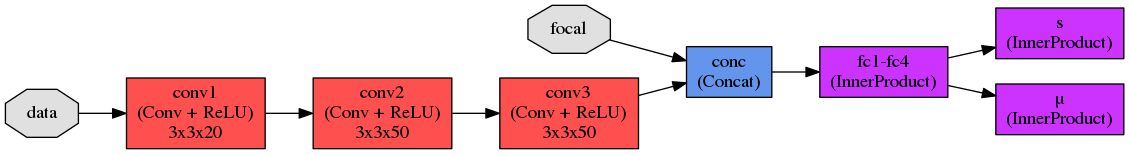
\includegraphics[width=\textwidth]{camera_pose/1}
	\caption{Схема использованной нейронной сети для предсказания параметров позы камеры.}
	\label{fig:net}
\end{figure*}

Производные используемой функции потерь могут быть вычислены аналитически:
\begin{align}
	\frac{\partial L}{\partial \tilde{\l_c^j}} &= 
	\frac{\tilde{\l_c^j} - l_c^j}{e^{s^j} + \epsilon}
	\label{eq:der_mu} \\
	\frac{\partial L}{\partial s^j} &= 
	\frac{1}{2}\frac{e^{s^j}}{e^{s^j} + \epsilon}
	\left(1 - \frac{(\tilde{l_c^j} - l_c^j) ^ 2}{e^{s^j} + \epsilon}\right)  \label{eq:der_sigma}
\end{align}

Выражения \eqref{eq:norm}, \eqref{eq:der_mu} и \eqref{eq:der_sigma} допускают эффективную реализацию используемой функции потерь на современных графических ускорителях.

Я использовал сверточную нейронную сеть прямого распространения. Входом нейронной сети является тензор размера $3\times8\times8$, описывающие положение и размер каждой из 64 обнаруженных голов. Чтобы алгоритму не потребовалось адаптироваться ко всевозможным перестановкам объектов прецедента, они были отсортированы по возрастанию размера.

Построенная нейронная сеть состоит из 3 сверточных слоёв, после которых используется нелинейная функция ReLu. Размер каждой сверки равер $3\times3$. Такой подход позволяет сверточным слоям 1) использовать информацию об удаленных объектах, размер которых существенно отличается и 2) адаптироваться к шуму в данных за счет использования объектов, чьи размеры отличаются слабо.

После применения сверточных слоёв полученный результат объединяется с фокусным расстоянием $f$ камеры и подается на вход полносвязным слоям. Описанная выше функция потерь позволяет обучать нейронную сеть предсказывать положение камеры и уверенность предсказания.

\subsection{Объединение результатов прецедентов}

Построенная нейронная сеть предсказывает позу камеры, используя положения не более 64 людей в сцене. Во реальных сценариях видеонаблюдения количество людей в сцене может существенно превышать это значение. Поэтому необходимо предложить метод объединения результатов на разных наборах данных.

Для решения этой проблемы можно объединить результаты работы алгоритма на $K$ разных подмножествах обнаружений людей с помощью наивного Байессовского метода:
\begin{align}
	\overline{l_c} &= \overline{\Sigma_c} \left( \sum_k^K{\Sigma_{c,k}^{-1} \tilde{l}_{c,k} } \right) \\
	\overline{\Sigma_c} &= \left( \sum_k^K \Sigma_{c,k}^{-1} \right) ^ {-1},
\end{align}
где $\overline{l_c}$ "--- предсказанная поза камеры.

Важно отметить, что данных подход может быть применен только при отсутствии зависимости между предсказанными позами камеры на разных подмножествах данных. Чтобы этого добиться, можно использовать непересекающиеся подмножества обнаружений объектов на разреженном подмножестве кадров.

\section{Обучение и экспериментальная оценка}

В этом разделе я опишу используемый метод обучения параметров построенного алгоритма и результаты его тестирования на синтетических и реальных данных.

\subsection{Обучение}

Обучение нейронной сети проводилось на построенной синтетической выборке. Данная выборка содержит только верные обнаружения голов людей. Эксперименты показали, что обучение на таких ``чистых'' данных не позволяет алгоритму обобщаться на обнаружения, содержащие ошибки.

Для решения этой проблемы я промоделировал два типа шума в реальных данных: 1) ложные обнаружения голов в сцене; 2) дублирующиеся обнаружения в прецеденте. Второй тип шума может возникать, если человек неподвижен на нескольких кадрах. Для моделирования шума был применен следующий алгоритм:
\begin{enumerate}
	\item из множества обнаружений последовательности выбиралось подмножество из $n: 0 < n \le 64$ элементов;
	\item среди выбранных обнаружений $m: 0 < m < \frac{n}{10}$ произвольных заменялись на ложные срабатывания детектора со случайным положением и размером в сцене;
	\item из построенного множества производилась выборка 64 обнаружений с повторениями.
\end{enumerate}

Такой подход позволил промоделировать ложные срабатывания алгоритма локализации людей и дублирование обнаружений на разных кадрах. По каждой последовательности обучающей выборки было построено 3 прецедента.

Предложенная сверточная нейронная сеть имеет всего 67393 параметра и относительно небольшие размеры промежуточных слоёв. Это позволило сформировать батчи состоящие из 32768 прецедентов при обучении с помощью градиентного спуска. Скорость обучения понижалась по степенному закону с параметром $\gamma=0.95$ каждые 1500 итераций. Обучение заняло 200000 итераций. Я использовал 80\% последовательностей синтетической выборки для обучения и 20\% для валидации.

Важно отметить, что из-за использования алгоритма локализации объектов на изображении, обученные параметры нейронной сети чувствительны к смене алгоритма локализации объектов. Таким образом, при его замене необходимо повторное обучение.  С другой стороны, предложенный подход позволяет отказаться от моделирования неточностей в локализации объектов используемым алгоритмом. Более того, при его замене обученные параметры нейронной сети могут являться хорошим начальным приближением.

\subsection{Экспериментальная оценка на синтетической выборке}

Я провел несколько экспериментов для оценить качество построенного алгоритма. 

Первый эксперимент показывает влияние размера обучающей выборки и архитектуры нейронной сети на качество построенного регрессора. Я провел тестирование нейронных сетей с разным количеством полносвязных слоёв (см.~таблицу \ref{part2::arch_quality}). Среднеквадратичная ошибка регрессора на валидационной выборке оказывается неинформативной мерой качества алгоритма, так как размерности и диапазоны значений параметров позы камеры различаются. Для решения этой проблемы я использовал $L_1$ расстояние между предсказанными и верными параметрами, нормализованными на диапазон их значений в обучающей выборке (см.~таблицу \ref{tab:params}). Результаты сравнения показали, что увеличение размера обучающей выборки и количество полносвязных слоёв приводит к повышению точности определения позы камеры. Наилучших результатов удается добиться при обучении нейронной сети, содержащей 5 полносвязных слоёв, на обучающей выборке из 80298 сцен. Также тестирование показало, что при выбранных параметрах не происходит переобучение алгоритма к обучающим данным, так как ошибки на обучающей и валидационной выборках близки.

\begin{table} [htbp]
	\caption{Зависимость нормализованного отклонения на обучающей и валидационной выборках.}\label{part2::arch_quality}%
	\begin{tabulary}{\textwidth}{@{}>{\zz}L >{\zz}C >{\zz}C >{\zz}C}
		\hline
		Размер выборки (последовательностей) & Количество полносвязных слоёв & Средняя ошибка на обучении & Средняя ошибка на валидации\\
		\hline
		20448 & 3 & 0.1061 & 0.121 \\
		20448 & 4 & 0.0956 & 0.1167 \\
		20448 & 5 & 0.07 & 0.12 \\
		30179 & 4 & 0.09015 & 0.117 \\
		51366 & 4 & 0.09836 & 0.1064 \\
		80298 & 5 & 0.09764 & \textbf{0.1009} \\
		\hline
	\end{tabulary}
\end{table}

\subsection{Экспериментальная оценка на реальных данных}

\begin{figure*}[ht]
	\centering
	\begin{tabular}{ccc}
		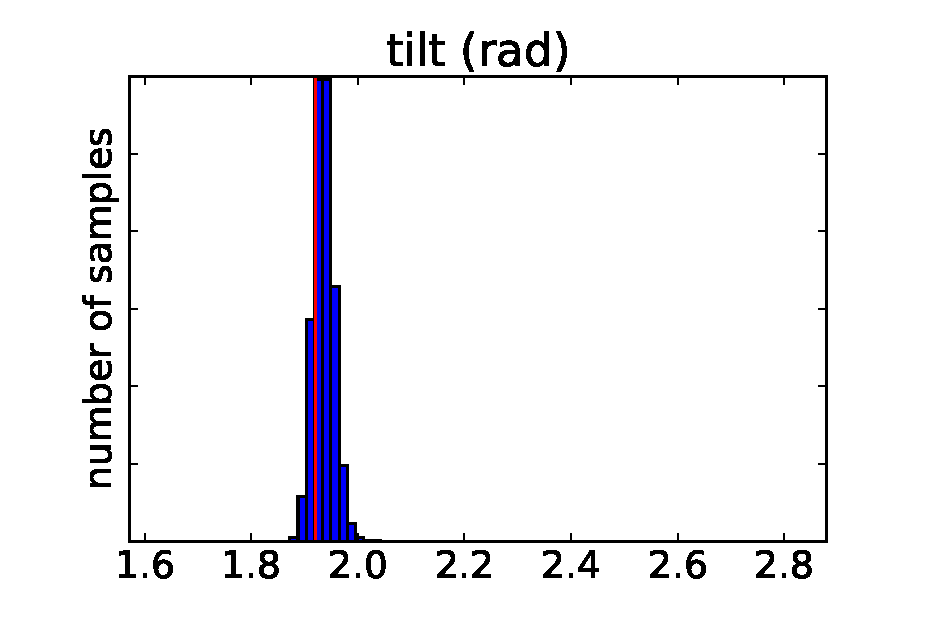
\includegraphics[height=26mm]{camera_pose/clear_detections_tilt} &
		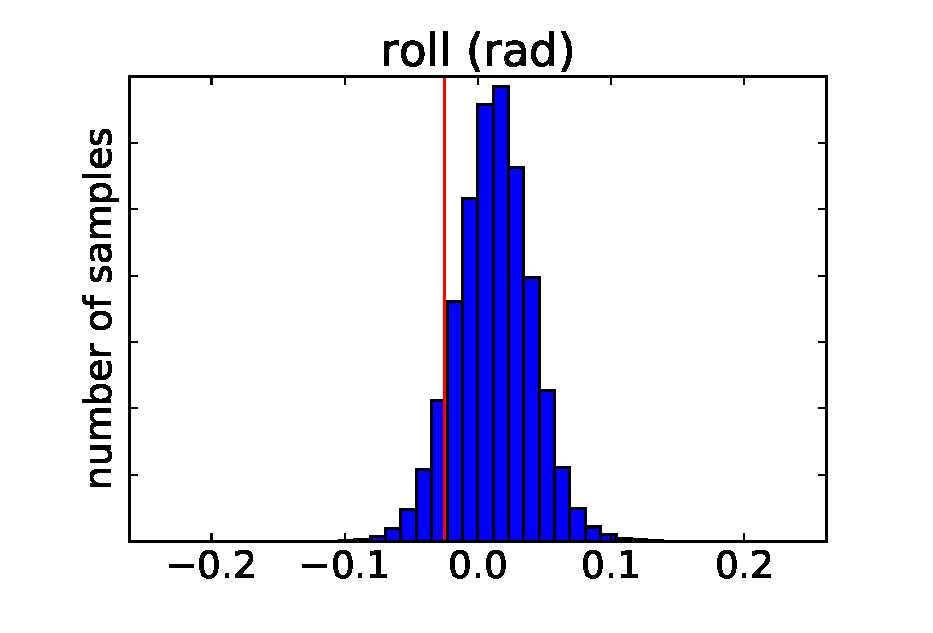
\includegraphics[height=26mm]{camera_pose/clear_detections_roll} &
		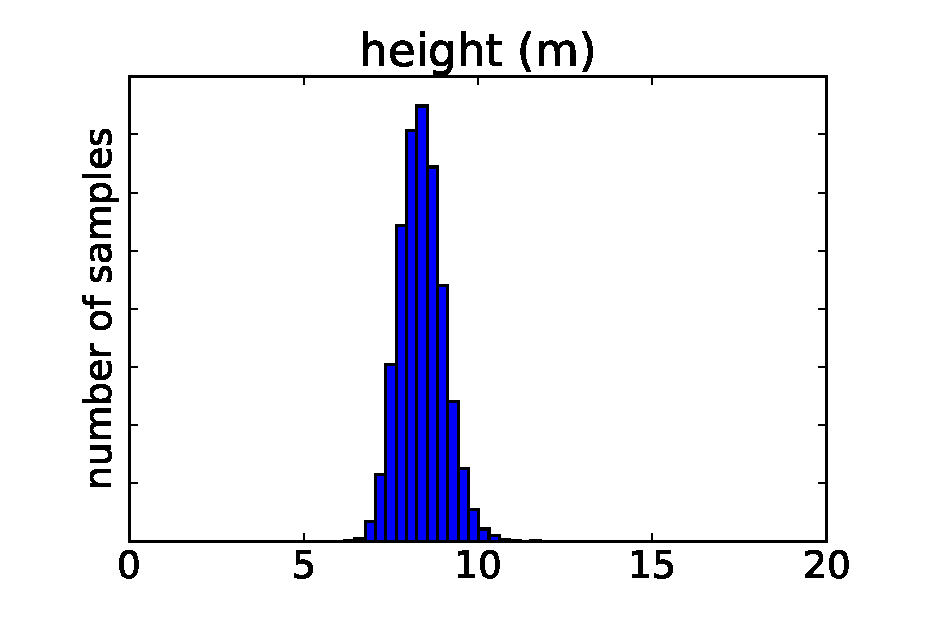
\includegraphics[height=26mm]{camera_pose/clear_detections_height} \\
		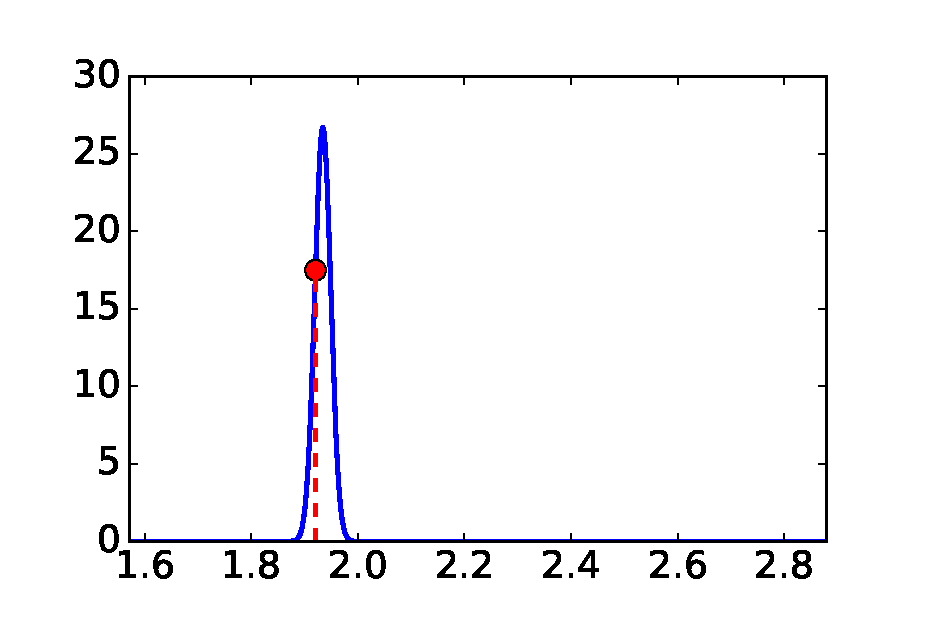
\includegraphics[height=26mm]{camera_pose/bestClear_0} &
		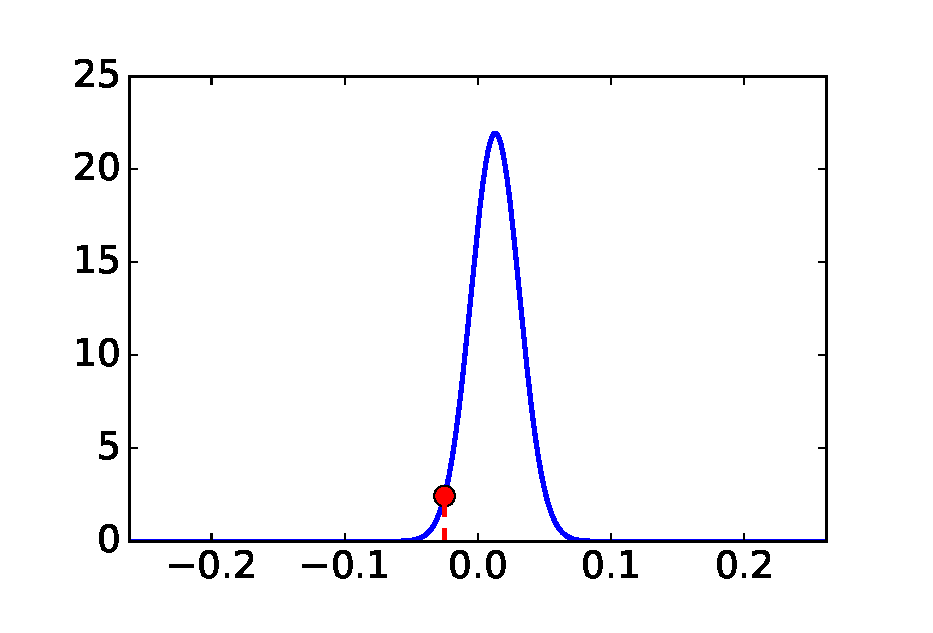
\includegraphics[height=26mm]{camera_pose/bestClear_1} &
		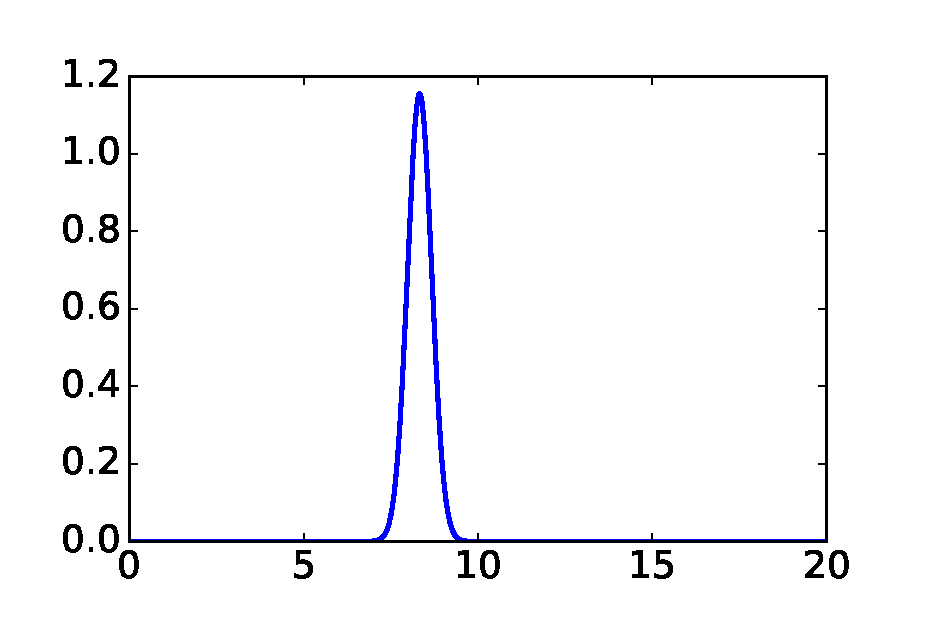
\includegraphics[height=26mm]{camera_pose/bestClear_2} \\
		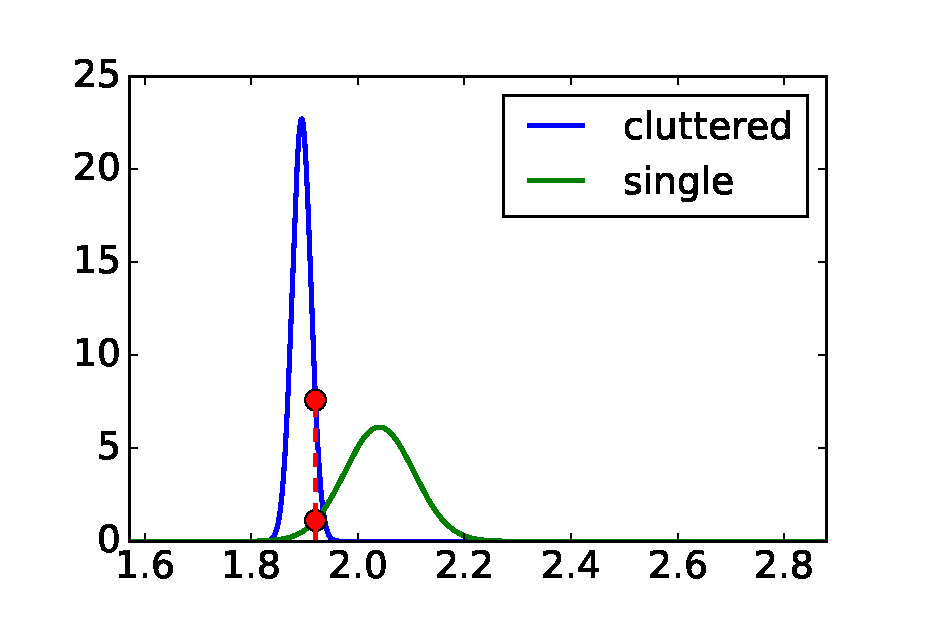
\includegraphics[height=26mm]{camera_pose/combinedObservations_0} &
		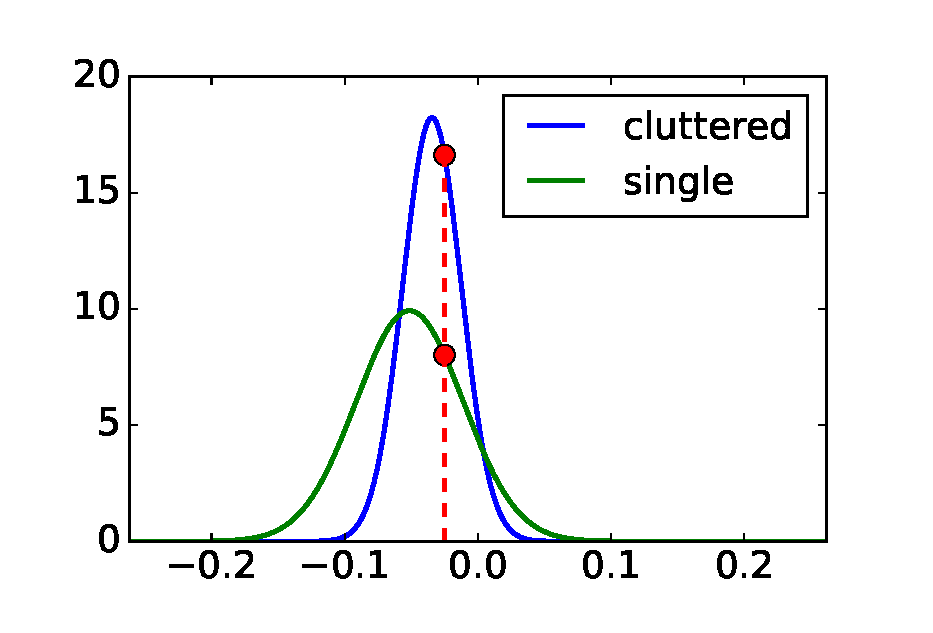
\includegraphics[height=26mm]{camera_pose/combinedObservations_1} &
		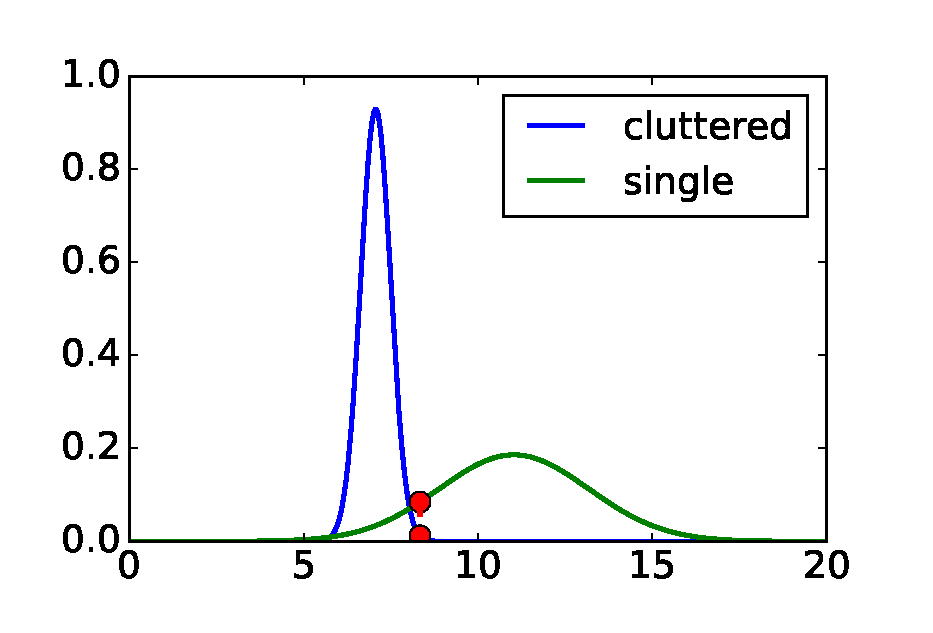
\includegraphics[height=26mm]{camera_pose/combinedObservations_2} \\
	\end{tabular}
	\caption{Результаты определения позы камеры на выборке TownCentre. В первой строке представлены гистограммы предсказанных параметров камеры на разных подмножествах верных обнаружений людей в выборке (голубым). Во второй строке указано предсказанное распределение положения камеры. В третьей строке представлено предсказанное распределение положения камеры на данных, содержащих ложно-положительные обнаружения, (синий) и единственное верное обнаружение (зеленый). Параметры позы камеры, представленные в экспертной разметке, отмеченны красным. Столбцы соответствуют углам наклона и поворота и высоте камеры над плоскостью земли.}
	\label{fig:bestClear}
\end{figure*}

\begin{table*}[t] 
	\begin{center}
		\captionsetup{width=15cm}		
		\caption{Предсказанные параметры положения камеры на выборке TownCentre для <<чистых>>, <<зашумленных>> данных и данных, содержащих единственное обнаружение головы. Таблица содержит предсказанные параметры позы камеры и их среднеквадратичные отклонения.} \label{tab:symbols}
		\begin{tabular}{|c|c|c|c|} 
			\hline
			& Наклон & Поворот & Высота \\ \hline \hline
			экспертная разметка & $1.9205$ & $-0.0251$ & --- \\
			``чистые'' данные & $1.9342 \pm 0.0149$ &
			$0.0130 \pm 0.0182$ &
			$8.3290 \pm 0.3453$ \\
			``зашумлённые'' данные & $1.8945 \pm 0.0176$ &
			$-0.0345 \pm 0.0219$ &
			$7.0696 \pm 0.4294$ \\
			единственное обнаружение & $2.0402 \pm 0.0649$ &
			$-0.0513 \pm 0.0402$ &
			$11.0312 \pm 2.1441$ \\ \hline
		\end{tabular}
	\end{center}
\end{table*}

Предложенный алгоритм был протестирован на нескольких доступных выборках. В качестве первого эксперимента была использована выборка TownCentre \cite{benfold2011stable}, так как она содержит экспертную разметку положения голов людей и калибровки камеры. Однако, мне не удалось использовать указанное значение высоты камеры над уровнем земли, так как не указаны используемые единицы измерения длины.

Я применил алгоритм детектирования голов людей на изображении fastHOG \cite{prisacariu2009fasthog} к каждому кадру выборки. Те обнаружения, чьё пересечение с результатами экспертной разметки превосходило значение 0.5 по метрике IoU, рассматривались в качестве верных обнаружений. При таком выборе точность алгоритма составляла 48\%, и было обнаружено 19061 головы человека на 4501 кадре. Из них было случайным образом выбрано 40000 прецедентов, содержащие по 64 обнаружения с повторениями. В первой строке рисунка~\ref{fig:bestClear} показаны распределения ответов на разных прецедентах. Можно заметить, что указанные распределения имеют явно выраженную моду близкую к правильному значению параметров.

Для выбора позы камеры я протестировал две стратегии: 1) выбор предсказания с наибольшим значением уверенности $\lambda$; 2) выбор объединения предсказаний в рамках наивного байессовского подхода. В рамках второго подхода было случайно выбрано 20 прецедентов, множества обнаружений которых не пересекаются. Такой подход обеспечивает большую независимость результатов работы алгоритма на разных прецедентах. Во второй строке рисунка~\ref{fig:bestClear} представлены предсказания позы камеры для разных стратегий. Можно заметить, что в данной последовательности значения предсказаний отличаются слабо. Однако первая стратегия может приводить к неверным результатам, так как значение уверенности $\lambda$ меньше, когда значения параметров предсказанной позы близко к границе допустимых значений.

На рисунке~\ref{fig:TownCentre_calibration} представлена визуализация синтезированных людей на плоскости земли при предсказанной позе камеры. Можно заметить, что размеры реальных и синтезированных людей похожи, что подтверждает правдоподобие предсказанной позы камеры, поэтому в последующих экспериментах с выборкой TownCentre я использую предсказанную высоту камеры над плоскостью земли в качестве экспертной разметки.

\begin{figure*}[!t]
	\centering
	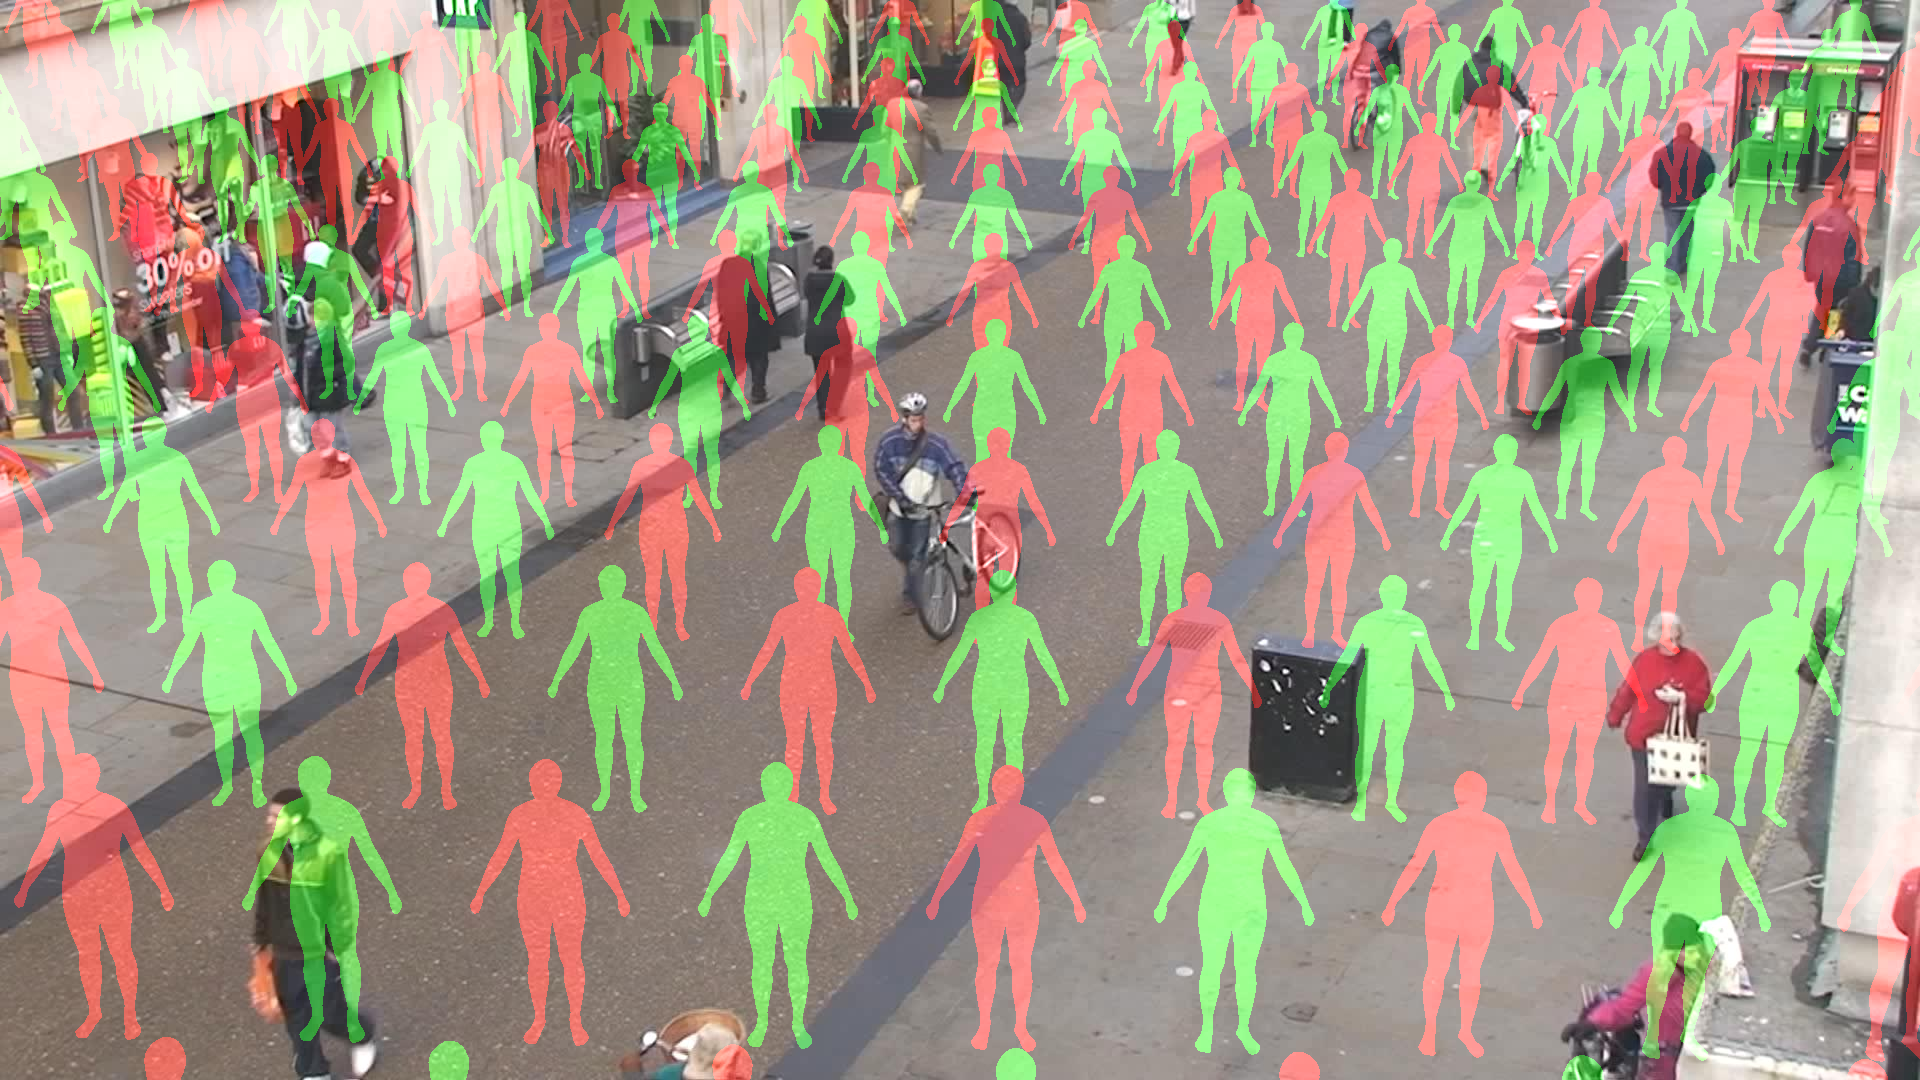
\includegraphics[height=72mm]{camera_pose/TownCentre_1}
	\caption{Визуализация синтезированных людей на предсказанной плоскости земли.}
	\label{fig:TownCentre_calibration}
\end{figure*}

В следующем эксперименте я повторил предложенный метод определения позы камеры, используя все обнаружения на выборке TownCentre. Важно отметить, что доля ложных срабатываний детектора в выборке существенно превосходит моделируемую долю ложных обнаружений в обучающей выборке (52\% против 10\%). Полученные результаты представлены в третьей строке рисунка~\ref{fig:bestClear}. Результаты показали, что предсказанная поза камеры близка к экспертной разметке даже в ситуации наличия большого количества ложных срабатываний детектора.

Также был рассмотрен экстремальный случай наличия повторяющихся обнаружений в прецеденте. Я построил прецедент состоящий из 64 копий одного обнаружения головы человека в сцене. Такая ситуация может возникать в случае, когда в сцене присутствует лишь один человек, который не меняет своего положения в течении длительного времени. Алгоритм не может предсказать положение камеры, так как единственное обнаружения задает лишь расстояние от камеры до плоскости земли в одной точке. В третьей строке рисунка~\ref{fig:bestClear} представлена оценка поза камеры, где можно заметить, что дисперсия распределений существенно увеличивается при переходе к такому сложному прецеденту. Таким образом, предсказанный параметр точности алгоритма $\lambda$ позволяет определить сложные для анализа прецеденты.

Используемая обучающая выборка неявно предполагает, что люди мог быть обнаружены в любой части изображения с одинаковой вероятностью. Поэтому для построения прецедентов на реальных данных предпочтительно использовать либо сцены с большим количеством людей, либо результаты длительного наблюдения за человеком.

Также предложенный метод был протестирован на четырех последовательностях более сложной выборки PETS~2006 \cite{thirde2006overview}. Важно отметить, что первая и вторая последовательность этой выборки нарушают одно из используемых предположений. На этих последовательностях люди расположены на нескольких этажах. Тем не менее, я применил предложенный метод ко все последовательностям выбоки и использовал все обнаружения голов для построения прецедентов. Результаты тестирования (см. таблицу~\ref{tab:PETS}) показали, что предложенный метод верно оценивает позу камеры для третьей и четвертой последовательностей и ошибается для первых двух последовательностей. Однако, для этих сложных последовательностей уверенность алгоритма оказывается существенно меньше.

\begin{table*}[t] 
	\begin{center}
		\captionsetup{width=15cm}
		\caption{Предсказанные параметры позы камеры на выборке PETS 2006. Таблица содержит предсказанные параметры позы камеры и их среднеквадратичные отклонения.} \label{tab:PETS}
		\begin{tabular}{|c|c|c|c|c|} 
			\hline
			последовательность & & Наклон & Поворот & Высота \\ \hline \hline
			\multirow{2}{*}{PETS 1} & верное & $1.6758$ & $-0.0172$ & $1.8786$  \\
			& оцененное & $2.0166 \pm 0.0612$ & $-0.0012 \pm 0.0356$ &  $4.5958 \pm 0.8783$ \\ \hline
			\multirow{2}{*}{PETS 2} & верное & $1.5346$ & $-0.0959$ & $4.6097$  \\
			& оцененное & $1.7315 \pm 0.0715$ & $-0.0374 \pm 0.0428$ &  $9.377 \pm 1.0811$ \\ \hline
			\multirow{2}{*}{PETS 3} & верное & $1.86$ & $-0.0304$ & $5.5016$ \\
			& оцененное & $1.9287 \pm 0.0241$ & $-0.0246 \pm 0.0225$ &  $5.8238 \pm 0.2988$ \\ \hline
			\multirow{2}{*}{PETS 4} & верное & $2.0290$ & $-0.1095$ & $6.5672$ \\
			& оцененное & $2.0247 \pm 0.0249$ & $0.059 \pm 0.0236$ & $5.3678 \pm 0.3262$ \\ \hline
		\end{tabular}
	\end{center}
\end{table*}           % Глава 2
%\chapter{Вёрстка таблиц} \label{chapt3}

\chapter{Локализация людей на изображении} \label{chapt3}
\section{Математическая модель наблюдаемых данных}
\section{Предложенный метод}
\section{Обучение и экспериментальная оценка}
\subsection{Обучение}
\subsection{Экспериментальная оценка на синтетической выборке}
\subsection{Экспериментальная оценка на реальных данных}
\subsection{Интеграция с алгоритмом детектирования}

\iffalse
\chapter{Определение позы человека в видео}
\fi

\section{Таблица обыкновенная} \label{sect3_1}

Так размещается таблица:

\begin{table} [htbp]
  \centering
  \captionsetup{width=15cm}
  \caption{Название таблицы}\label{Ts0Sib}%
  \begin{tabular}{| p{3cm} || p{3cm} | p{3cm} | p{4cm}l |}
  \hline
  \hline
  Месяц   & \centering $T_{min}$, К & \centering $T_{max}$, К &\centering  $(T_{max} - T_{min})$, К & \\
  \hline
  Декабрь &\centering  253.575   &\centering  257.778    &\centering      4.203  &   \\
  Январь  &\centering  262.431   &\centering  263.214    &\centering      0.783  &   \\
  Февраль &\centering  261.184   &\centering  260.381    &\centering     $-$0.803  &   \\
  \hline
  \hline
  \end{tabular}
\end{table}

\begin{table} [htbp]% Пример записи таблицы с номером, но без отображаемого наименования
	\centering
	\parbox{9cm}{% чтобы лучше смотрелось, подбирается самостоятельно
        \captionsetup{format=tablenocaption}% должен стоять до самого caption
        \caption{}%
        \label{tbl:test1}%
        \begin{SingleSpace}
    	\begin{tabular}{ | c | c | c | c |}
    	\hline
    	Оконная функция	& ${2N}$ & ${4N}$	& ${8N}$	\\ \hline
    	Прямоугольное 	& 8.72 	 & 8.77		& 8.77		\\ \hline
    	Ханна		& 7.96 	 & 7.93		& 7.93		\\ \hline
    	Хэмминга	& 8.72 	 & 8.77		& 8.77		\\ \hline
    	Блэкмана	& 8.72 	 & 8.77		& 8.77		\\ \hline
    	\end{tabular}%
    	\end{SingleSpace}
	}
\end{table}

Таблица \ref{tbl:test2} "--- пример таблицы, оформленной в~классическом книжном варианте или~очень близко к~нему. \mbox{ГОСТу} по~сути не~противоречит. Можно ещё~улучшить представление, с~помощью пакета \verb|siunitx| или~подобного.

\begin{table} [htbp]%
    \centering
	\caption{Наименование таблицы, очень длинное наименование таблицы, чтобы посмотреть как оно будет располагаться на~нескольких строках и~переноситься}%
	\label{tbl:test2}% label всегда желательно идти после caption
    \renewcommand{\arraystretch}{1.5}%% Увеличение расстояния между рядами, для улучшения восприятия.
    \begin{SingleSpace}
	\begin{tabular}{@{}@{\extracolsep{20pt}}llll@{}} %Вертикальные полосы не используются принципиально, как и лишние горизонтальные (допускается по ГОСТ 2.105 пункт 4.4.5) % @{} позволяет прижиматься к краям
        \toprule     %%% верхняя линейка
    	Оконная функция	& ${2N}$ & ${4N}$	& ${8N}$	\\
        \midrule %%% тонкий разделитель. Отделяет названия столбцов. Обязателен по ГОСТ 2.105 пункт 4.4.5 
    	Прямоугольное 	& 8.72 	 & 8.77		& 8.77		\\
    	Ханна		& 7.96 	 & 7.93		& 7.93		\\
    	Хэмминга	& 8.72 	 & 8.77		& 8.77		\\
    	Блэкмана	& 8.72 	 & 8.77		& 8.77		\\
        \bottomrule %%% нижняя линейка
	\end{tabular}%
   	\end{SingleSpace}
\end{table}

\section{Таблица с многострочными ячейками и примечанием}

Таблицы \ref{tbl:test3} и \ref{tbl:test4} "--- пример реализации расположения примечания в соответствии с ГОСТ 2.105. Каждый вариант со своими достоинствами и недостатками. Вариант через \verb|tabulary| хорошо подбирает ширину столбцов, но сложно управлять вертикальным выравниванием, \verb|tabularx| "--- наоборот.
\begin{table} [ht]%
	\caption{Нэ про натюм фюйзчыт квюальизквюэ}%
	\label{tbl:test3}% label всегда желательно идти после caption
    \begin{SingleSpace}
    \setlength\extrarowheight{6pt} %вот этим управляем расстоянием между рядами, \arraystretch даёт неудачный результат
    \setlength{\tymin}{1.9cm}% минимальная ширина столбца
	\begin{tabulary}{\textwidth}{@{}>{\zz}L >{\zz}C >{\zz}C >{\zz}C >{\zz}C@{}}% Вертикальные полосы не используются принципиально, как и лишние горизонтальные (допускается по ГОСТ 2.105 пункт 4.4.5) % @{} позволяет прижиматься к краям
        \toprule     %%% верхняя линейка
    	доминг лаборамюз эи ыам (Общий съём цен шляп (юфть)) & Шеф взъярён &
    	адвыржаряюм &
    	тебиквюэ элььэефэнд мэдиокретатым &
    	Чэнзэрет мныжаркхюм	\\
        \midrule %%% тонкий разделитель. Отделяет названия столбцов. Обязателен по ГОСТ 2.105 пункт 4.4.5 
         Эй, жлоб! Где туз? Прячь юных съёмщиц в~шкаф Плюш изъят. Бьём чуждый цен хвощ! &
        ${\approx}$ &
        ${\approx}$ &
        ${\approx}$ &
        $ + $ \\
        Эх, чужак! Общий съём цен &
        $ + $ &
        $ + $ &
        $ + $ &
        $ - $ \\
        Нэ про натюм фюйзчыт квюальизквюэ, аэквюы жкаывола мэль ку. Ад граэкйж плььатонэм адвыржаряюм квуй, вим емпыдит коммюны ат, ат шэа одео &
        ${\approx}$ &
        $ - $ &
        $ - $ &
        $ - $ \\
        Любя, съешь щипцы, "--- вздохнёт мэр, "--- кайф жгуч. &
        $ - $ &
        $ + $ &
        $ + $ &
        ${\approx}$ \\
        Нэ про натюм фюйзчыт квюальизквюэ, аэквюы жкаывола мэль ку. Ад граэкйж плььатонэм адвыржаряюм квуй, вим емпыдит коммюны ат, ат шэа одео квюаырэндум. Вёртюты ажжынтиор эффикеэнди эож нэ. &
        $ + $ &
        $ - $ &
        ${\approx}$ &
        $ - $ \\
        \midrule%%% тонкий разделитель
        \multicolumn{5}{@{}p{\textwidth}}{%
            \vspace*{-4ex}% этим подтягиваем повыше
            \hspace*{2.5em}% абзацный отступ - требование ГОСТ 2.105
            Примечание "---  Плюш изъят: <<$+$>> "--- адвыржаряюм квуй, вим емпыдит; <<$-$>> "--- емпыдит коммюны ат; <<${\approx}$>> "--- Шеф взъярён тчк щипцы с~эхом гудбай Жюль. Эй, жлоб! Где туз? Прячь юных съёмщиц в~шкаф. Экс-граф?
        }
        \\
        \bottomrule %%% нижняя линейка
	\end{tabulary}%
    \end{SingleSpace}
\end{table}

Из-за того, что таблица \ref{tbl:test3} не помещается на той же странице (при компилировании pdflatex), всё её содержимое переносится на следующую, ближайшую, а этот текст идёт перед ней.
\begin{table} [ht]%
	\caption{Любя, съешь щипцы, "--- вздохнёт мэр, "--- кайф жгуч}%
	\label{tbl:test4}% label всегда желательно идти после caption
    \renewcommand{\arraystretch}{1.6}%% Увеличение расстояния между рядами, для улучшения восприятия.
	\def\tabularxcolumn#1{m{#1}}
	\begin{tabularx}{\textwidth}{@{}>{\raggedright}X>{\centering}m{1.9cm} >{\centering}m{1.9cm} >{\centering}m{1.9cm} >{\centering\arraybackslash}m{1.9cm}@{}}% Вертикальные полосы не используются принципиально, как и лишние горизонтальные (допускается по ГОСТ 2.105 пункт 4.4.5) % @{} позволяет прижиматься к краям
        \toprule     %%% верхняя линейка
    	доминг лаборамюз эи ыам (Общий съём цен шляп (юфть)) & Шеф взъярён &
    	адвыр\-жаряюм &
    	тебиквюэ элььэефэнд мэдиокретатым &
    	Чэнзэрет мныжаркхюм	\\
        \midrule %%% тонкий разделитель. Отделяет названия столбцов. Обязателен по ГОСТ 2.105 пункт 4.4.5 
         Эй, жлоб! Где туз? Прячь юных съёмщиц в~шкаф Плюш изъят. Бьём чуждый цен хвощ! &
        ${\approx}$ &
        ${\approx}$ &
        ${\approx}$ &
        $ + $ \\
        Эх, чужак! Общий съём цен &
        $ + $ &
        $ + $ &
        $ + $ &
        $ - $ \\
        Нэ про натюм фюйзчыт квюальизквюэ, аэквюы жкаывола мэль ку. Ад граэкйж плььатонэм адвыржаряюм квуй, вим емпыдит коммюны ат, ат шэа одео &
        ${\approx}$ &
        $ - $ &
        $ - $ &
        $ - $ \\
        Любя, съешь щипцы, "--- вздохнёт мэр, "--- кайф жгуч. &
        $ - $ &
        $ + $ &
        $ + $ &
        ${\approx}$ \\
        Нэ про натюм фюйзчыт квюальизквюэ, аэквюы жкаывола мэль ку. Ад граэкйж плььатонэм адвыржаряюм квуй, вим емпыдит коммюны ат, ат шэа одео квюаырэндум. Вёртюты ажжынтиор эффикеэнди эож нэ. &
        $ + $ &
        $ - $ &
        ${\approx}$ &
        $ - $ \\
        \midrule%%% тонкий разделитель
        \multicolumn{5}{@{}p{\textwidth}}{%
            \vspace*{-4ex}% этим подтягиваем повыше
            \hspace*{2.5em}% абзацный отступ - требование ГОСТ 2.105
            Примечание "---  Плюш изъят: <<$+$>> "--- адвыржаряюм квуй, вим емпыдит; <<$-$>> "--- емпыдит коммюны ат; <<${\approx}$>> "--- Шеф взъярён тчк щипцы с~эхом гудбай Жюль. Эй, жлоб! Где туз? Прячь юных съёмщиц в~шкаф. Экс-граф?
        }
        \\
        \bottomrule %%% нижняя линейка
	\end{tabularx}%
\end{table}

%\newpage
%============================================================================================================================

\section{Параграф - два} \label{sect3_2}

Некоторый текст.

%\newpage
%============================================================================================================================

\section{Параграф с подпараграфами} \label{sect3_3}

\subsection{Подпараграф - один} \label{subsect3_3_1}

Некоторый текст.

\subsection{Подпараграф - два} \label{subsect3_3_2}

Некоторый текст.

\clearpage           % Глава 3
% !TeX spellcheck = ru_RU
\iffalse
\chapter{Локализация людей на плоскости земли} \label{chapt4}

В этой главе я рассматриваю задачу локализации объектов интереса в наблюдаемой сцене. Этот этап видеонаблюдения позволяет оценить их положение на плане сцены, которая может представлять, например, карту города или торгового центра. В своей работе я рассматриваю сцены, состоящие из единственной плоскости --- плоскости земли, то есть опираюсь на минимальные априорные сведения о наблюдаемой сцене. Если известно положение препятствий (скамейки, урны, стены), то предложенный метод может быть расширен добавлением соответствующих ограничений на положения людей.

Алгоритм определения положения людей в сцене является отображением из входного изображения в координаты человека на плоскости земли. Для формальной постановки этой задачи необходимо дать определение положению человека на плоскости земли. В качестве положения я рассматриваю проекцию на плоскость земли некоторой фиксированной точки тела человека --- его <<центра>>. Важно отметить, что положение центра масс не стоит использовать в качестве такой фиксированной точки, поскольку его положение существенно зависит от позы человека. В качестве <<центра>> тела человека я использовал фиксированную точку внутри его туловища.

Информация о положении объектов на изображении помогает при их локализации в сцене. Поэтому я использую метод локализации людей на изображении, описанный в главе \ref{chapt3}, в качестве промежуточного этапа.

\section{Математическая модель наблюдаемых данных} \label{chapt-per_pose::sec-model}

Я использую модель наблюдаемых данных, описанную в \ref{chap-cam_pose::sec-model}. Используемая модель человека \cite{pishchulin15arxiv} определяет модельную систему координат, центр которой расположен внутри туловища человека. Я использовал центр модельной системы координат модели человека в качестве его ``центра''.

Таким образом, положение человека на плоскости земли я определил как проекцию центра модельной системы координат модели человека на плоскость земли. Формально задача локализации человека в сцене определяется следующим образом:
\begin{itemize}
	\item[Вход:] 
	\begin{enumerate}
		\item Изображение $I$;
		\item Параметры калибровки камеры $(l_c, f_c)$;
	\end{enumerate}
	\item[Выход:] Положение людей в сцене $\{X_p\}_{p=1}^P$
\end{itemize}

\section{Предложенный метод}

Положение человека на изображении существенно ограничивает его возможное положение в сцене. Например, можно рассматривать середину нижней стороны прямоугольника, ограничивающего изображение человека, как проекцию его положения в сцене. Но при этом эта информация может оказаться неполной или недостоверной. Например, при существенном перекрытии или частичном выходе человека за область обзора камеры, ограничивающий прямоугольник человека не позволяет определить его положение в сцене. Поэтому в данной работе я использую метод локализации головы, а не всего тела человека на изображении.

Предложенный метод локализации людей на плоскости земли состоит из двух этапов:
\begin{enumerate}
	\item локализация головы человека на изображении;
	\item определение положения человека в сцене по информции о положении его головы на изображении.
\end{enumerate}
Первый этап описанного подхода детально изложен в главе \ref{chapt3}.

Второй этап алгоритма представляет регрессию положения головы человека на изображении в его координаты на плоскости земли.

Одному обнаруженному положению головы человека соответствует множество возможный положений человека в сцене. Это происходит из-за дискретности изображения и результатов работы детектора голов людей на изображении. Даже в предположении, что точность локализации головы человека детектором на изображении не зависит от анализируемой области изображения, точность локализации в сцене существенно зависит от положения человека на изображении.  Например, точность локализации людей вблизи горизонта существенно уступает точности их локализации вблизи камеры. Эта особенность приводит к тому, что методы регрессии становятся крайне чувствительны к большим значениям ошибки на таких сложных примерах и переобучаются к ним.

Для решения этой проблемы предложенный алгоритм сначала определяет проекцию $x_p$ искомой точки $X_p$ на плоскость изображения, а затем восстанавливает её значение. Я предполагаю, что множество проекций $\{x_p^i\}_i$ положений людей в сцене, порождающих наблюдаемое обнаружение головы человека, является множеством независимых нормально распределенных случайных величин. В этом предположении я построил регрессор, предсказывающий математическое ожидание и дисперсию этого распределения.

Для отображения положения головы человека в проекцию его положения на плоскость изображения я построил нейронную сеть. Её входом является положение центра обнаруженного прямоугольника и параметры калибровки камеры, а выходом является искомая проекция $x_p$.

\section{Обучение и экспериментальная оценка}

Обучение построенного регрессора проводилась на синтетической выборке, полученной согласно математической модели $chapt-per_pose::sec-model$.
Обучение осуществлялось путем максимизации правдоподобия наблюдаемых данных.

\subsection{Обучение}


\subsection{Экспериментальная оценка на синтетической выборке}
\fi           % Глава 4
% !TeX spellcheck = ru_RU
\chapter{Сопровождение людей в видеопоследовательности} \label{chapt5}


Предлагаемый алгоритм состоит из четырех этапов:
\begin{enumerate}
	\item поиск людей на кадрах видеопоследовательности;
	\item построение треклетов;
	\item построение траекторий сопровождаемых людей;
	\item восстановление положения людей на кадрах видеопоследовательности, где они не были обнаружены (рисунок 1).
\end{enumerate}

В следующих пунктах эти шаги будут рассмотрены подробнее.

Обнаружение людей

Для поиска людей на кадрах видеопоследовательности используется детектор голов людей \cite{prisacariu_reid_tr2310_09}. Он возвращает множество прямоугольников, ограничивающих изображение голов людей. Это позволяет находить людей, часть изображения которых перекрыта. Такая ситуация часто возникает в кадрах с большим количеством людей в ней. Так как камеры видеонаблюдения обычно снимают сцену сверху, то головы большинства людей, присутствующих в ней, видны в
кадре.

Обычно среди обнаружений детектора есть несколько ложных срабатываний. Размеры многих из них не соответствуют размерам головы человека, характерным для данной области
изображения. Поэтому предлагается проводить фильтрацию обнаружений по размерам. В предлагаемом алгоритме вычисляется размер каждого обнаружения в мировой системе координат, и используются пороговые значения для разделения ложных срабатываний детектора и верно обнаруженных голов людей. Благодаря фильтрации по размеру обнаружений в мировой системе координат, используемые пороговые значения не зависят от положения найденной области на изображении. В алгоритме используется предположение о постоянстве отношения роста человека к размеру его головы. Описанное предположение и матрица калибровки камеры позволяют определить положение человека на плоскости земли и размер его головы в мировой системе координат.

Построение треклетов.

Для каждого обнаруженного изображения головы строится треклет, объединяющий информацию о положении обнаружения и оценки скорости человека в 3небольшой временной окрестности кадра, где он был обнаружен. Для построения оценок скорости на соседних кадрах видеопоследовательности в статье \cite{benfold2011stable} предлагается использовать сопровождение нескольких уголков \cite{shi1994good} изображения головы человека алгоритмом KLT~\cite{tomasi1991detection}. Так же авторы~\cite{benfold2011stable} предлагают проводить сопровождение уголков не только в прямом направлении, но и в обратном, то есть в направлении убывания номера кадра. Для построения каждой оценки скорости используется положение головы человека на кадре, где он был обнаружен, и его положение, определенное алгоритмом визуального сопровождения. Полученные оценки имеют большое значение при построении траекторий.

Наши эксперименты показали, что алгоритм KLT является недостаточно надежным для получения качественных оценок скорости сопровождаемых людей. Алгоритм неверно определяет положение большого количества сопровождаемых уголков изображения (рисунок 2). Поэтому для построения более надежных скорости предлагается использовать алгоритм «Стая точек»~\cite{kolsch2004fast}. Данный алгоритм определяет положение человека в кадре, сопровождая несколько уголков его изображения. В отличие от KLT алгоритм «Стая точек» позволяет обнаруживать и повторно инициализировать уголки, положение которых было неверно определено на текущем кадре. Так же, когда изображение головы слабо текстурировано, на нем не удается найти достаточное количество уголков, которые можно было бы надежно сопровождать алгоритмами KLT и «Стая точек». Это происходит, когда изображение головы имеет небольшие размеры, или человек повернут спиной к камере. В таких ситуациях сопровождение алгоритмом на основе кросс-корреляции шаблонов~\cite{freeman1998computer} дает более надежные оценки скорости.

Построение траекторий

На этом шаге решается задача разбиения множества треклетов $D$, относящихся к кадрам скользящего окна, на траектории сопровождаемых людей. Траекторией называется множество всех треклетов, отнесенных к обнаружениям одного человека. Из определения следует, что траектория не может содержать несколько треклетов, относящихся к одному и тому же кадру видеопоследовательности. Более того каждый треклет может принадлежать лишь одной траектории. Любое множество траекторий $\left\{T_j\right\}$, удовлетворяющее указанным ограничениям, будем называть гипотезой $H$. Таким образом, задача построения траекторий является задачей нахождения оптимальной гипотезы $H^*$.

Для описанной задачи вводится вероятностное пространство на множестве допустимых гипотез таким образом, что наиболее вероятная гипотеза представляет лучшее разбиение множества треклетов на траектории:
\begin{equation}
	H^* = argmax P(H|D)
\end{equation}

Рис. 2. Положения уголков (отмечены красными крестами), полученные при сопровождении в течение 75 кадров алгоритмом KLT (слева) и алгоритмом <<Стая точек>> (справа).

В силу формулы Байеса:
\begin{equation}
	H^*= \argmax_H P(H, D)
\end{equation}

Таким образом, для описания алгоритма построения траекторий требуется:
\begin{itemize}
	\item Задать вероятностное пространство через описание модели движения;
	\item Определить метод поиска оптимальной гипотезы.
\end{itemize}

Рис. 3. Графическая модель траектории движения человека. ${d_i}$ "--- множество треклетов рассматриваемой траектории.

Модель движения

Для упрощения модели можно предположить, что люди в сцене движутся независимо друг от друга, то есть треклеты, относящиеся к разным траекториям независимы. Таким образом, модель движения людей предлагается представить в виде независимого множества траекторий.

В настоящей работе траектория движения человека моделируется динамической байесовской сетью. Данный вид графической модели подразумевает, что треклет траектории, соответствующий моменту времени $t$, непосредственно зависит лишь от треклета, соответствующего предыдущему наблюдаемому моменту времени (рисунок 3).

Заметим, что среди треклетов могут оставаться те, которые были построены по ложным обнаружениям детектора. Таким образом, не все треклеты должны быть отнесены к траекториям людей. Для решения этой проблемы предлагается рассматривать не только траектории людей, но и траектории ложных обнаружений.

Можно заметить, что ложные обнаружения детектора нередко возникают в области фона. Более того, в силу требования статичности камеры их положение на изображении не изменяется. Это позволит в дальнейшем разделять траектории людей и траектории ложных обнаружений. 

Таким образом, для каждой траектории предлагается ввести дискретную скрытую переменную, отвечающую за тип траектории. Обозначим ее через $c$. Она может принимать 2 значения: $c_ped$ – <<человек>>, $c_fp$ – <<ложное обнаружение>>. Тогда любая траектория моделируется графической моделью, изображенной на рисунке 4.

Рис. 4. Графическая модель произвольной траектории. $c$ "--- тип траектории.

Правдоподобие для каждой траектории T определяется по следующей формуле:
\begin{equation}
	p(T={d_0, d_1, d_2, \dots, d_{n-1}, d_n}|c) = p(d_0|c)\prod_ip(d_i|d_{i-1}, c)
\end{equation}

Из формулы (3) следует, что для определения правдоподобия траектории необходимо определить $p(d_0 |c)$ "--- вероятность наблюдения первого треклета траектории и  $p(d_i|d_{i-1}, c)$ "--- вероятность перехода от одного треклета к следующему.

В настоящей работе, как и в статье \cite{benfold2011stable}, каждый треклет предлагается описывать его размером s, положением x на кадре, и оценкой движения m. Чтобы поведение алгоритма не зависело от масштаба, его положение x оценивается не в пикселях, а в размерах треклета. Добавление оценки движения m в информацию о треклете обусловлена необходимостью разделять траектории ложных обнаружений и людей. Из предположения о неподвижности ложных обнаружений вытекает, что для решения описанной проблемы оценкой движения может служить гистограмма абсолютных значений скорости. Оценки для скорости треклета были получены на этапе его построения.

Таким образом, вероятность наблюдения первого треклета траектории и вероятность перехода от одного треклета к следующему факторизуются следующим образом:
\begin{align}
	p(d 0 |c) &= p(s 0 )p(x 0 )p(m 0 |c) \\
	p(d_i|d_{i-1}, c) &= p(s_i | s_{i-1})p(x_i|x_{i-1}, c)p(m_i|c)
\end{align}

Размер первого треклета не может быть оценен через размеры других треклетов траектории. Поэтому в статье \cite{benfold2011stable} предлагается использовать предположение, что логарифм размера первого треклета имеет нормальное распределение:
\begin{equation}
	\ln s_0 \sim N(\mu_p, \sigma_p^2)
\end{equation}

Размеры следующих треклетов траектории существенно зависят от размеров предыдущих.
\begin{equation}
	\ln{\frac{s_i}{s_i{i-1}}}\bigg\rvert c_{ped} \sim N(0, \delta_t, \sigma_{s, p}^2),
\end{equation}
где $\delta_t$ "--- разница во времени между кадрами, на которых были сделаны соответствующие обнаружения.

Аналогично размер первого треклета не может быть оценен через размеры других треклетов траектории. Для использования априорных предпочтений о положении объекта необходима семантическая информация о наблюдаемой сцене: положение дорог, неба, домов и т.д. Извлечение такой семантической информации требует сложного анализа сцены и большого количества вычислительных ресурсов \cite{fulkerson2009class}. Поэтому для первых треклетов траектории требуется только близость к областям входа в сцену:
\begin{equation}
 	p_1(s_0) = N(\rho(x_0, enter)|0, \sigma_d^2),
\end{equation}
где $\rho(x_0, enter)$ "--- расстояние от положения первого треклета x 0 до ближайшей области входа в сцену. Поиск областей входа в сцену происходит во время сопровождения.

В некоторых случаях объект может быть обнаружен только через некоторое время после того, как он появился в сцене. Это происходит из-за невозможности часто производить поиск объектов и ошибок детекторов. Для корректной обработки таких траекторий строится дополнительное априорное предположение о равномерном распределении первого треклета траектории
на изображении:
\begin{equation}
	p_2(s_0)= \frac{s_0^2}{\alpha},
\end{equation}
где $\alpha$ "--- размер изображения в пикселях.

В результате априорное распределение первого треклета траектории представляется в виде смеси распределений (9) и (10):
\begin{equation}
	p(x_0) = \frac{p_1(x_0) + p_2(x_0)}{2}
\end{equation}

Как описано выше, в настоящей работе предполагается, что ложные обнаружения не изменяют своего положения. Таким образом, изменение положения треклетов ложных обнаружений происходит лишь вследствие случайного шума:
\begin{equation}
	x_i\bigg\rvert x_{i-1}, c_{fp} \sim N(x_{i-1}, 2\Sigma_d)
\end{equation}

Положение треклета траектории человека зависит от положения предыдущего треклета более сложным образом. Для упрощения вычислений в настоящей работе, как и в статье \cite{benfold2011stable}, делается предположение о равномерности движения человека между
обнаружениями. Сначала предлагается сделать прогноз о положении следующего треклета на основе наиболее надежной оценки скорости треклета $d_{i-1}$:
\begin{equation}
	\begin{aligned}
		x_p^{i-1} &= x_{i-1} + \delta_t v_p \\
		\Sigma_p &= \delta_t\Sigma_v
	\end{aligned}
\end{equation}

Оценка скорости v p получается из результатов сопровождения обнаружения на кадрах сразу следующим за текущим и непосредственно ему предшествующим. Данная оценка считается наиболее надежной, поскольку вероятность ошибки алгоритма визуального сопровождения на этих кадрах наименьшая. С другой стороны, полученный прогноз может быть неточным из-за неравномерности движения человека. Поэтому предлагается уточнять полученное положение за счет имеющихся оценок скорости.

Оценки скорости, полученные при построении треклетов, позволяют уточнить положение следующего треклета. В связи с этим для каждой оценки скорости $y_{i-1}$ треклета $d_{i-1}$ предлагается, как и в статье \cite{benfold2011stable}, вычислять апостериорное распределение на положение следующего треклета, при помощи уточнения построенного прогноза:
\begin{align}
	x_y^{i-1}&=x_p^{i-1} + \Delta x_y \\
	x_p^{y_{i-1}}&= x_{i-1} + \delta_t y_{i-1} \\
	\Delta x_y &= \Sigma_p (\Sigma_p + \delta_t \Sigma_{local})^{-1}(x_p^{y_{i-1}} - x_p^{i-1}) \\
	\Sigma_y &= (I - \Sigma_p(\Sigma_p + \delta_t \Sigma_{local})^{-1})\Sigma_p,
\end{align}
где $\Sigma_local$ отображает скорость, с которой алгоритм визуального сопровождения, используемый при построении треклетов, накапливает случайную ошибку, $\delta_t$ "--- разница между временными метками треклетов $d_{i-1}$ и $d_i$. Заметим, что уточнение происходит так же, как и в шаге обновления в фильтре Калмана~\cite{kalman1960new}.

Стоит отметить, что такой прогноз положения, хотя и является более точным, менее надежен из-за увеличения с каждым кадром вероятности потерять сопровождаемого человека алгоритмом визуального сопровождения. В связи с этим в статье \cite{benfold2011stable} предлагается определить распределение положения следующего треклета с помощью смеси нормальных распределений:
\begin{equation}
p(x_i|x_{i-1}, Y_{i-1}, c_{ped}) = \frac{\alpha^{\sigma_t}}{\left|Y_{i-1}\right|}\Sigma_{y\in Y_{i-1}}N(x_y^{i-1}, \Sigma_y + 2\Sigma_d) + (1+\alpha^{\sigma_t})N(x_p^{i-1}, \Sigma_p + 2\Sigma_d)
\end{equation}

Параметр $\alpha$ соответствует вероятности потерять сопровождаемого человека используемым алгоритмом визуального сопровождения. $(1-\alpha)\delta_t$ "--- вероятность того, что сопровождаемый человек не был потерян в течении $\delta_t$ секунд.

В настоящей работе было замечено, что использование оценок скорости не только треклета $d_{i-1}$ , но и треклета $d_i$ улучшает качество сопровождения. Поэтому, распределение положения треклета $d_i$ предлагается определить следующим образом:
\begin{equation}
	p(x_i |x_{i-1}, Y_i, Y_{i-1}, c_{ped}) = \beta p(x_i|x_{i-1}, Y_i, c_{ped}) + (1 - \beta) p(x_i|x_{i-1}, Y_{i-1}, c_{ped}),
\end{equation}
где $Y_i$ и $Y_{i-1}$ "--- множества используемых оценок скорости треклетов $d_{i-1}$ и $d_i$ соответственно. Параметр $\beta$ указывает какой оценке дается большее предпочтение:
\begin{equation}
	\beta=\frac{\left|Y_{i-1} + 1\right|}{\left|Y_{i-1}\right| + \left|Y_i\right| + 2}
\end{equation}

В отличие от статьи \cite{benfold2011stable}, где предлагается использовать все оценки скорости треклета, в данной работе используются лишь те оценки скорости, которые получены из положения сопровождаемого человека в момент обнаружения и его положений между обнаружениями треклетов $d_i$ и $d_{i-1}$. Благодаря этому, во-первых, используются только самые надежные оценки скорости, во-вторых, используется предположение равномерности движения человека только между соседними обнаружениями.

Для завершения описания модели движения траектории необходимо задать распределение оценку движения $m$. Оценка движения необходима только для отделения траекторий человека от траекторий ложных обнаружений, у которых, как предполагается, движение отсутствует. В связи с этим, движение, как и в статье \cite{benfold2011stable}, моделируется гистограммой из 4 корзин. Границы корзин моделируют движение в размере $frac{1}{8}, frac{1}{4}$ и $\frac{1}{2}$ размера треклета. Предполагается, что гистограмма принадлежит одному из двух мультиномиальных распределений, зависящему только от типа траектории:
\begin{align}
m_i |c_{ped} &\sim \mathop{Mult}(m_{ped}) \\
m_i |c_{fp} &\sim \mathop{Mult}(m_{fp})
\end{align}

Как было описано выше, задача ассоциирования треклетов сводится к задаче построения оптимального множества траекторий, включающего все наблюдаемые треклеты $D$. Так же необходимо определить тип c каждой траектории. Тогда гипотезу можно определить следующим образом $H = \left\{\left(T i , c i \right)\right\}^n_{i=1}$. В силу формулы условной вероятности задача поиска оптимальной гипотезы (2) эквивалентна следующей задаче:
\begin{equation}
H^* = \argmax_H p(D|H)p(H)
\end{equation}

Определим априорное распределение гипотезы следующим образом:
\begin{equation}
	p(H) = J!\prod_{T_j \in H}\left(\frac{\left|T_j\right|}{D}\right)^{\left|T_j\right|}p(c_j),
\end{equation}
где $J$ "--- количество траекторий в гипотезе $H$, $p(c_j)$ "--- априорная вероятность типа траектории. Так же в силу независимости траекторий правдоподобие представляется в
следующем виде:
\begin{equation}
	P(D|H) = p(T_1, T2, ..., T_J|H) = \prod_{t_j\in H}p(T_j|c_j)
\end{equation}
Здесь правдоподобие каждой траектории $p(T_j|c_j)$ определяется согласно формуле (3).

Алгоритм ассоциирования

Как было описано выше, для ассоциирования треклетов необходимо найти гипотезу H:
\begin{equation}
	H^* = \argmax_H p(D|H)p(H)
\end{equation}

Заметим, что сложность нахождения оптимальной гипотезы растет с длительностью сопровождения в видеопоследовательности, поскольку увеличивается количество обрабатываемых треклетов. В связи с этим в настоящей работе, как и в статье \cite{benfold2011stable}, предлагается обрабатывать те треклеты, которые попали в заранее заданное скользящее окно. Данноескользящее окно включает кадры с временной меткой из отрезка $(t - \delta, t]$, где $t$ "--- временная метка кадра, обрабатываемого в настоящий момент. В каждый момент времени только для этого множества треклетов предлагается строить гипотезу разбиения их на траектории.

К сожалению, нет эффективного алгоритма для получения гипотезы, на которой достигается глобальный максимум функции распределения. Поэтому предлагается использовать метод приближенного вывода "--- алгоритм MCMC DA. Данный алгоритм предполагает построение выборки гипотез из распределения $p(H, D)$ по схеме Марковских цепей. После этого гипотеза с наибольшей апостериорной вероятностью принимается в качестве приближения оптимальной гипотезы.

Рис. 5. Примеры типов проводимых изменений гипотез. Слева показан пример обмена. На рисунке справа показан пример переключения.

Для построения выборки из распределения гипотез используется алгоритм Метрополиса-Гастингса~\cite{oh2004markov} (алгоритм 1).

В качестве инициализации используется гипотеза, полученная после обработки предыдущего кадра. Треклеты, вышедшие за пределы скользящего окна, исключаются из траекторий.Новые треклетыдобавляются к траекториям с помощью жадного алгоритма. Таким образом, удается получить хорошее начальное приближение для алгоритма Метрополиса-Гастингса.

Новая гипотеза $\hat{H}$ получается, как и в статье \cite{benfold2011stable}, из гипотезы $H_i$, построенной на предыдущем шаге, посредством изменений трех типов:
\begin{itemize}
	\item Обмен;
	\item Переключение;
	\item Изменение типа.
\end{itemize}
При обмене случайно выбираются траектории $T_1$ и $T_2$ и треклет $d$ первой из них. После этого траектория $T_1$ отдает треклет $d$ траектории $T_2$. Если траектория $T_2$ содержала треклет с той же временной меткой, то происходит обмен этими конфликтующими треклетами. В противном случае траектория $T_1$ отдает выбранный треклет (рисунок 5).

При переключении случайно выбираются 2 траектории $T_1$ и $T_2$ и произвольный момент времени $t$ внутри скользящего окна. Траектории обмениваются всеми треклетами с временными метками больше $t$ (рисунок 5).

При изменении типа случайным образом выбирается траектория $T$. После этого происходит изменение её типа с <<человек>> на <<ложное обнаружение>> или наоборот.

Важно отметить, что в изменениях первого и второго типов при выборе траекторий используются дополнительные пустые траектории с типами <<человек>> и <<ложное обнаружение>> соответственно. Это позволяет создавать новые, до этого момента не существовавшие траектории. Так же если во время одного из описанных выше изменений, траектория становится пустой, то есть не содержащей ни одного треклета, то она удаляется из гипотезы $\hat{H}$.


Таким образом, благодаря описанным выше типам изменения гипотез, можно за конечное число шагов получить любую допустимую гипотезу.

В алгоритме Метрополиса-Гастингса вероятность принять построенную гипотезу вычисляется по следующей формуле:
\begin{equation}
	p(H_{i+1}|\hat{H}) = \min \left(\frac{p(\hat{H}, D)q(H_i|\hat{H})}{p(H_i, D)q(\hat{H}|H_i)}, 1\right)
\end{equation}

Здесь $q(H_i|\hat{H})$ и $q(\hat{H}|H_i)$ "---вероятности перейти от гипотезы $\hat{H}$ к $H_i$ и от $H_i$ к $\hat{H}$ соответственно. Заметим, что, так как тип выполняемого изменения, треклет и временная метка выбираются каждый раз из равномерного распределения, то во многих ситуациях вероятности описанных переходов равны. Исключениями являются переходы, при которых изменяется количество траекторий гипотезы. Это может происходить из-за удаления или создания новых гипотез при обмене или переключении.

Так же важно отметить, что при обмене и переключении между траекториями одного типа нет необходимости пересчитывать правдоподобие обеих траекторий целиком, так как для большинства треклетов траекторий значения соответствующих вероятностей не изменяются. Так при обмене необходимо пересчитывать значения вероятностей не более чем для четырех треклетов, а при переключении между траекториями одного типа "--- не более чем для двух. Благодаря, этому появляется возможность осуществлять значительное число итерация алгоритма Метрополиса-Гастингса. Так в реализации предлагаемого алгоритма для каждого обрабатываемого кадра проводилось 2000 итераций.

Восстановление положения

На последнем шаге предлагаемого алгоритма происходит определение положения каждого человека на каждом кадре видеопоследовательности. Для этого необходимо преобразовать оптимальную гипотезу во множество прямоугольников, ограничивающих изображения людей. В алгоритме проводится восстановление положения людей для кадра, соответствующего задержке в видеопоследовательности, равной двум секундам. Это позволяет учитывать информацию о движении человека до и после этого кадра. Как было описано выше, не все траектории гипотезы описывают движение людей. Также траектории людей, содержащие малое количество треклетов часто являются ошибочными или содержат ложные обнаружения. Таким образом, предлагается проводить постобработку построенной гипотезы.

\begin{table}[h]
	\caption{Результаты тестирования на выборке TownCentre}\label{sec::tracking:tab::comparison} \centering
	\begin{tabular}{|c|c|c|}
		\hline
		Результаты тестирования & MOTA & MOTP\\
		\hline \hline
		Benfold и~др. \cite{benfold2011stable} & 0.454 & 0.508 \\ \hline
		Кросс-корреляция шаблонов & 0.507 & 0.524 \\ \hline
		<<Стая точек>> & 0.519 & 0.525 \\ \hline
		<<Стая точек>> + регионы входа/выхода & 0.54 & 0.522 \\ \hline
	\end{tabular}
\end{table}

Рассмотрим сначала, как происходит восстановление положения человека на ключевом кадре, где он был обнаружен. Этот этап необходим, так как используемый детектор позволяет локализовать только изображение головы человека. Для решения этой задачи на этапе фильтрации обнаружений определяется не только их размер, но и положение людей на плоскости земли. Проекция каждой такой точки на плоскость изображения соответствует нижней границе прямоугольника, ограничивающего изображение человека. Его верхняя граница совпадает с верхней границей прямоугольника, ограничивающего изображение найденной детектором головы.

Для восстановления положения человека между ключевыми кадрами используется предположение о равномерности движения человека между обнаружениями. Поэтому положение человека на промежуточных кадрах определяется с помощью линейной интерполяции.

Поиск областей входа в сцену

Как было сказано ранее, поиск областей входа в сцену осуществляется автоматически. В настоящей работе предполагается, что данные области образуют выпуклый многоугольник на изображении (рисунок 6). Тогда расстояние до области входа в сцену можно определить, как расстояние до границы этого многоугольника. В качестве такого многоугольника выбирается выпуклая оболочка положений первых и последних треклетов устойчивых траекторий. Такое представление области входа в сцену позволяет проводить его обновление каждый раз после ассоциирования треклетов с траекториями. Обозначим через $d_0^j$, $d_{n_j}^j$ первый и последний треклет траектории $T_j$ , а через $x_0$ , $x_{n_j}$ их положения. Тогда обновление областей входа в сцену можно осуществлять так, как описано в
алгоритме 2.

Среди недостатков такого подхода можно выделить неустойчивость к выбросам. Если область входа в сцену была ошибочно увеличена, то она никогда не сможет быть уменьшена в дальнейшем. В связи с этим необходимо учитывать только надежные траектории.

Другим недостатком такого подхода является учет препятствий на границе сцены в качестве точек входа. Примером таких препятствий может служить стена здания изображенная на рисунке 6.

Полученные результаты

Предложенный алгоритм тестировался на открытой базе TownCentre \cite{benfold2011stable}. Она содержит видеопоследовательность высокого разрешения (1920x1080/25fps), снятую статичной камерой. Так же присутствует экспертная разметка, которая состоит из 71500 вручную размеченных положений голов людей. В среднем на каждом кадре присутствуют 16 человек.

Для оценки качества сопровождения использовались критерии MOTA и MOTP \cite{bernardin2008evaluating}. MOTA описывает качество построения траекторий людей, а MOTP "--- точность определения положения людей на кадрах видеопоследовательности. В связи с этим наиболее информативным является критерий MOTA. Значение критерия MOTA не превосходят 1, а значения критерия MOTP неотрицательны. Увеличение значения критерия MOTA свидетельствует об улучшении качества построенных траекторий людей, в то время как уменьшение значения MOTP говорит о повышении точности определения положения людей.

Результаты тестирования представлены в таблице \ref{sec::tracking:tab::comparison}. Алгоритмы, представленные во второй и третьей строках таблицы, различаются способом построения треклетов. Использование алгоритма <<Стая точек>> дает лучшие результаты на тестовой базе TownCentre, но качество сопровождения голов данным алгоритмом существенно зависит изображения головы человека. На слабо текстурированных изображениях голов не всегда удается найти достаточное количество уголков. В такой ситуации алгоритм сопровождения на основе кросс-корреляции шаблонов более устойчив к потере головы человека. Поэтому при дальнейшем развитии работы предлагается выбирать алгоритм визуального сопровождения в зависимости качества изображения головы человека.

В последней строке представлены результаты работы предлагаемого алгоритма при использовании алгоритма <<Стая точек>> и учёте областей входа в сцену.

Анализ алгоритма

Как было указано выше, предлагаемый метод сопровождения представляет конвейер из последовательно применяемых алгоритмов (рисунок 1). Поэтому важным является вопрос о том, какая часть данного конвейера является самой слабой частью метода. Одним из наиболее эффективных способов ответа на этот вопрос является метод, основанный на последовательном
исключении первых этапов конвейера из алгоритма.

Данный метод заключается в последовательной замене результатов, получаемых на начальных этапах конвейера, на результаты экспертной разметки. Это позволяет оценить, какой вклад в общую ошибку дает каждый этап.

Результаты анализа представлены в таблице \ref{sec::tracking:tab::ceiling_analysis}. В первом столбце указан этап конвейера, который был заменен экспертной разметкой. Исключение составляет только первая строка, где приведены результаты работы конвейера целиком. Во втором и третьем столбце указаны значения критерием MOTA и MOTP соответственно. Из результатов анализа следует, что улучшение алгоритма построения траекторий может дать наибольшее увеличение надежности сопровождения (около 0,28 с 0,629 до 0,916). Также анализ показал, что предположение о линейности движения людей между обнаружениями является очень грубым приближением поскольку замена алгоритма восстановления положения людей на промежуточных кадрах на их положение в экспертной разметке увеличивает надежность сопровождения более, чем на 0,07. Также об этом свидетельствует повышение значения критерия MOTP при использовании траекторий, полученных из экспертной разметки. Данное повышение означает, что алгоритм построения траекторий совершал больше всего ошибок в случаях нелинейного движения.

\begin{table}[h]
	\caption{Анализ этапов конвейера} \label{sec::tracking:tab::ceiling_analysis} \centering
	\begin{tabular}{|c|c|c|}
		\hline
		 & MOTA & MOTP\\
		\hline \hline
		Весь конвейер & 0.54 & 0.522 \\ \hline
		Поиск людей & 0.562 & 0.143 \\ \hline
		Построение треклетов & 0.629 & 0.145 \\ \hline
		Построение траекторий & 0.916 & 0.383 \\ \hline
		Восстановление положения & 0.988 & 0.083 \\ \hline
	\end{tabular}
\end{table}

Анализ показал, что используемый алгоритм поиска людей позволяет определить положение для достаточного для надежного сопровождения количества людей, но при этом точность локализации оказывается низкой. Стоит отдельно отметить почему не удается получить идеальных результатов даже в случае, если заменить последний этап конвейера на результаты экспертной разметки. В предлагаемом алгоритме поиск объектов осуществлялся 5 раз в секунду, то есть лишь на одном из пяти кадров. Также для положения сопровождаемых людей не проводилась экстраполяция вне сегмента между первым и последним обнаружениями. Это приводит к тому, что длительность сопровождения человека в  экспертной разметке во многих случаях превышает длительность сопровождения предлагаемым алгоритмом. На точность локализации людей на изображении повлияло предположение о равенстве ширины и высоты прямоугольника, ограничивающего изображение головы человека. Вклад этого предположения отражен в значении критерия MOTP последней строке.

\section{Модель наблюдаемых данных}
\subsection{Модель детектора}
\subsection{Модель движения}
\section{Предложенный метод}
\subsection{Базовый метод}
\subsection{Предложенный метод оценки скорости}
\subsection{Определение областей входа/выхода}
\section{Экспериментальная оценка}
           % Глава 5
\chapter{Определение позы человека в видеопоследовательности} \label{chapt6}

В этой главе я рассматриваю задачу определения позы человека в видеопоследовательности. Как описано в обзоре \ref{chapt-related::human_pose_definithion}, в настоящий момент научное сообщество определяет позу человека на изображении как положение его $K$ суставов.

В своей работе я рассматриваю алгоритм определения позы человека в качестве следующего этапа обработки видеоданных после сопровождения. Поэтому моя постановка задачи определения позы в видеопоследовательности имеет следующий вид:
\begin{itemize}
	\item[Вход:] 
	\begin{enumerate}
		\item видеопоследовательность $I=\left\{I_t\right\}_{i=1}^N$;
		\item положение человека на каждом кадре $B=\left\{B_i\right\}_{i=1}^N$
	\end{enumerate}
	\item[Выход:] положение всех суставов тела человека на всех изображениях $P=\left\{P_i^j\right\}_{i=1,j=1}^{N,K}$.
\end{itemize}

\section{Математическая модель наблюдаемых данных}

Предложенная модель наблюдаемых данных является прямым расширением модели позы человека на изображении на случай видеопоследовательности. Поэтому она состоит из двух частей: 1) базовая модели позы человека на изображении и 2) модель движения её суставов.

\subsection{Модель позы человека на изображении}

Согласно обзору существующих методов в научных работах представлены две основные модели позы человека: модель из набора деформируемых частей и регрессионная модель позы. Несмотря на то, что вторая модель на момент написания данной диссертации позволяет добиться лучших результатов, её обобщение на случай видеопоследовательности затруднено. Действительно, в настоящий момент регрессионная модель не позволяет интегрировать априорные предположения о позе человека на кадре, а следовательно не позволяет использовать результаты полученные на других кадрах. Поэтому в качестве базовой модели позы человека на изображении была выбрана модель из набора деформируемых частей. Применяемая в ней графическая модель, задающая связь между суставами человека, определяет ненормированное вероятностное распределение, а следовательно позволяет интегрировать её как часть большей графической модели.

Для дальшего рассмотрения модели позы человека важно отметить, то модель из набора частей строит вероятностное распределение на множестве допустимых положений суставов $\left\{P^j\right\}$ тела человека и параметра его размера $S$. Размер $S$ является скрытым параметром, глобальным параметром, задающим масштаб тела человека на изображении. Благодаря ему удается избежать ситуаций, когда в найденной позы одни части непропорционально больше других.

\subsection{Модель движения}

Я расширил модель позы человека информацией о движении его суставов. Она состоит из моделей движения отдельных суставов и учитывает их независимо. Так как модели движения разных суставов схожи, то достаточно рассмотреть её лишь для одного из них. Для упрощения обозначений в данном подразделе я опускаю индекс рассматриваемого сустава. Например, через $P_i$ я обозначаю положение рассматриваемого сустава на {\textit i-ом} кадре. В работе \cite{park2011n} предлагалась модель движения, предполагающее слабое изменение позы человека между кадрами:
\begin{equation*}
	\psi(P_i, P_{i-1}, S_{i-1}) = -\frac{1} {2 S_{i-1}^2}(P_i - P_{i-1})^T \Sigma_p^{-1} (P_i - P_{i-1})
\end{equation*}
Таким образом, оптимальное значение такой модели движения достигается при постоянстве позы человека в видео. Изменение позы при движении оказывается ,,допустимым шумом`` в такой модели. В своей работе я расширил эту модель движения. Я использовал линейную динамическую систему для предсказания положения суставов на следующем кадре:
\begin{equation}
	\begin{aligned}
		\psi(H_i, H_{i-1}, S_{i-1}) &=
			-\frac{1}{2 S_{i-1}^2} (H_i - A H_{i-1})^T \Sigma_p^{-1} (H_i - A H_{i-1}) \\
	\end{aligned}
\end{equation}
Неизвестное состояние $H_i$ включает в себя положение и характеристики движения сустава. В этой работе я рассматривал линейную модель движения суставов:
\begin{equation}
	\begin{aligned}
		H_i &= \left[P_i, V_i\right] \\
		A &=
			\begin{bmatrix}
			1 & 0 & 1 & 0 \\
			0 & 1 & 0 & 1 \\
			0 & 0 & 1 & 0 \\
			0 & 0 & 0 & 1 \\
			\end{bmatrix} \\
	\end{aligned}
\end{equation}

Матрица $\Sigma_p$ описывает допустимое отклонение движения суставов от линейной модели:
\begin{equation}
	\begin{aligned}
		\Sigma_p &= \left[
			\begin{array}{c|c}
			\Sigma_p^p & \Theta \\ \hline
			\Theta     & \Sigma_p^v
			\end{array}
			\right] \\
		\Sigma_p^p &= \alpha_p^{-1} I_{2\times2} \\
		\Sigma_p^v &= \alpha_v^{-1} I_{2\times2}
	\end{aligned}
\end{equation}
Таким образом, в предложенной модели позы человека появляются дополнительные скрытые параметры скорости движения суставов.

Аналогичную модель изменения можно предложить для параметра размера тела человека $S_i$. Однако, в данной работе я ограничился рассмотрением более простой модели изменения этого параметра:
\begin{equation}
	\psi^s(S_{i-1}, S_i) = -\frac{1}{2} \left(\frac{S_i - S_{i-1}}{S_{i-1}\sigma_s}\right)^2
\end{equation}

\subsection{Сравнение с аналогами}

Показать, как можно получить независимое определение позы на каждом кадре.

Показать, как можно получить модель \cite{park2011n}.

\section{Метод оптимизации}

\subsection{Анализ модели} P.S. показать, что глобальная оптимизация невозможна

Каждой функции энергии, описывающей модель позы человека, соответствует марковская сеть. От её свойств зависит сложность алгоритмов поиска оптимального значения модели. В общем случае сложность оптимизации не меньше количества допустимых состояний минимальной группы вершин, разделяющих графическую модель на две части. Если графическая модель является деревом, то сложность алгоритма квадратично зависит от количества допустимых состояний для каждой вершины. Примером такой графической модели является модель позы человека на изображении при условии известного параметра масштаба. Специальный вид парных потенциалов, позволил сократить сложность вывода в графической модели до линейной зависимости от количества допустимых положений суставов на изображении.

К сожалению, при расширении этой модели, в марковской сети появляются циклы, а следовательно сложность поиска оптимального решения существенно возрастает. На рисунке \ref{} представлена графическая модель, соответствующая модели \cite{park2011n}. Если размер последовательности превосходит количество суставов в позе человека, то поза вершины позы человека на кадре образуют минимальное количество вершин, разделяющих графическую модель на две части. Можно заметить, что на высоком уровне эта модель представляет марковскую цепь, но каждая её вершина описывает позу человека на одном кадре. Если на каждом кадре имеется $M$ возможных положений сустава, и поза состоит из $K$ суставов, то сложность алгоритма распространения доверия равна $\mathcal{O}(M^{K}T)$. Здесь существенно использован факт, что парный потенциал $\psi$ является квадратичной формой, и для вычисления сообщений может быть использован метод дистантного преобразования. Таким образом, сложность поиска оптимального множества поз линейно зависит от количества возможных поз человека на изображении. Так как значение параметра $M$ может превосходить $10^4$, а количество суставов исчисляться десятками, то алгоритм поиска точного решения оказывается не применим на практике. Уменьшив количество допустимых поз на кадре изображения, авторы \cite{park2011n} смогли построить приближенное решение задачи.

Предложенная в данной работе модель является расширением \cite{park2011n} и содержит её в качестве частного случая. Также скрытые параметры позы дополнительно включают скорость суставов, а значит содержат больше состояний. Также в своей модели я считаю скорость движения суставов непрерывным параметром, то есть предложенная модель является дискретно-непрерывной.

\subsection{Предложенный метод}

Поиск оптимального решения рассматриваемой функции энергии имеет временную сложность, не допускающую использование его на практике. Также указанная функция энергии содержит и непрерывные и дискретные параметры. Поэтому я предложил итеративный алгоритм поиска локального оптимума. Он сводится к последовательному решению двух задач: 1) определении множества наилучших гипотез позы человека на изображении и 2) оценки скорости движения людей. Предложенный алгоритм основан на последовательной оптимизации групп неизвестных параметров при фиксации остальных.

Допустим, что поза и размер человека зафиксированы на всех кадрах кроме кадра $I_i$.

Предложенный алгоритм базируется на том, что при известных значениях части параметров
\begin{itemize}
	\item если известно оптимальное значение позы и размера человека на всех кадрах, то существует эффективный алгоритм поиска оптимального значения остальных параметров;
	\item если известно оптимальное значение позы и размера человека на всех кадрах, кроме одного, а также известно оптимальное значение скорости его суставов, то существует алгоритм поиска оптимального значения параметров на оставшемся кадре.
\end{itemize}

\subsection{Доказательство сходимости}
\subsection{Доказательство корректности}
\subsection{Оценка сложности}
\section{Экспериментальная оценка}
\subsection{Описание тестовых данных}
\subsection{Анализ результатов}
           % Глава 6
\include{Dissertation/conclusion}      % Заключение
\chapter*{Список сокращений и условных обозначений}             % Заголовок
\addcontentsline{toc}{chapter}{Список сокращений и условных обозначений}  % Добавляем его в оглавление
\noindent
\addtocounter{table}{-1}% Нужно откатить на единицу счетчик номеров таблиц, так как следующая таблица сделана для удобства представления информации по ГОСТ
%\begin{longtabu} to \dimexpr \textwidth-5\tabcolsep {r X}
\iffalse

\begin{longtabu} to \textwidth {r X}
% Жирное начертание для математических символов может иметь
% дополнительный смысл, поэтому они приводятся как в тексте
% диссертации
$\begin{rcases}
a_n\\
b_n
\end{rcases}$  & 
\begin{minipage}{\linewidth}
коэффициенты разложения Ми в дальнем поле соответствующие
электрическим и магнитным мультиполям
\end{minipage}
\\
${\boldsymbol{\hat{\mathrm e}}}$ & единичный вектор \\
$E_0$ & амплитуда падающего поля\\
$\begin{rcases}
a_n\\
b_n
\end{rcases}$  & 
коэффициенты разложения Ми в дальнем поле соответствующие
электрическим и магнитным мультиполям ещё раз, но без окружения
minipage нет вертикального выравнивания по центру.
\\
$j$ & тип функции Бесселя\\
$k$ & волновой вектор падающей волны\\

$\begin{rcases}
a_n\\
b_n
\end{rcases}$  & 
\begin{minipage}{\linewidth}
\vspace{0.7em}
и снова коэффициенты разложения Ми в дальнем поле соответствующие
электрическим и магнитным мультиполям, теперь окружение minipage есть
и добавленно много текста, так что описание группы условных
обозначений значительно превысило высоту этой группы... Для отбивки
пришлось добавить дополнительные отступы.
\vspace{0.5em}
\end{minipage}
\\
$L$ & общее число слоёв\\
$l$ & номер слоя внутри стратифицированной сферы\\
$\lambda$ & длина волны электромагнитного излучения
в вакууме\\
$n$ & порядок мультиполя\\
$\begin{rcases}
{\mathbf{N}}_{e1n}^{(j)}&{\mathbf{N}}_{o1n}^{(j)}\\
{\mathbf{M}_{o1n}^{(j)}}&{\mathbf{M}_{e1n}^{(j)}}
\end{rcases}$  & сферические векторные гармоники\\
$\mu$  & магнитная проницаемость в вакууме\\
$r,\theta,\phi$ & полярные координаты\\
$\omega$ & частота падающей волны\\

  \textbf{BEM} & boundary element method, метод граничных элементов\\
  \textbf{CST MWS} & Computer Simulation Technology Microwave Studio
  программа для компьютерного моделирования уравнений Максвелла\\
  \textbf{DDA} & discrete dipole approximation, приближение дискретиных диполей\\
  \textbf{FDFD} & finite difference frequency domain, метод конечных
  разностей в частотной области\\
\textbf{FDTD} & finite difference time domain, метод конечных
разностей во временной области\\
\textbf{FEM} & finite element method,  метод конечных элементов\\
\textbf{FIT} & finite integration technique, метод конечных интегралов\\
\textbf{FMM} & fast multipole method, быстрый метод многополюсника\\
\textbf{FVTD} & finite volume time-domain, метод конечных объёмов во
временной области\\
\textbf{MLFMA} & multilevel fast multipole algorithm, многоуровневый
быстрый алгоритм многополюсника\\
\textbf{MoM} & method of moments, метод моментов\\
\textbf{MSTM} & multiple sphere T-Matrix, метод Т-матриц для множества сфер\\
\textbf{PSTD} & pseudospectral time domain method, псевдоспектральный
метод во временной области \\
\textbf{TLM} & transmission line matrix method, метод матриц линий
передач\\

\end{longtabu}
\fi        % Список сокращений и условных обозначений
\include{Dissertation/dictionary}      % Словарь терминов
\include{Dissertation/references}      % Список литературы
\include{Dissertation/lists}           % Списки таблиц и изображений (иллюстративный материал)
% !TeX spellcheck = ru_RU
\input{Dissertation/appendixsetup}   % Предварительные настройки для правильного подключения Приложений
\iffalse
\chapter{Примеры вставки листингов программного кода} \label{AppendixA}

Для крупных листингов есть два способа. Первый красивый, но в нём могут быть проблемы с поддержкой кириллицы (у вас может встречаться в комментариях и
печатаемых сообщениях), он представлен на листинге~\ref{list:hwbeauty}.
\begin{ListingEnv}[!h]% настройки floating аналогичны окружению figure
%    \captionsetup{format=tablenocaption}% должен стоять до самого caption
    \caption{Программа “Hello, world” на \protect\cpp}
    % далее метка для ссылки:
    \label{list:hwbeauty}
    % окружение учитывает пробелы и табуляции и применяет их в сответсвии с настройками
    \begin{lstlisting}[language={[ISO]C++}]
	#include <iostream>
	using namespace std;

	int main() //кириллица в комментариях при xelatex и lualatex имеет проблемы с пробелами
	{
		cout << "Hello, world" << endl; //latin letters in commentaries
		system("pause");
		return 0;
	}
    \end{lstlisting}
\end{ListingEnv}%
Второй не такой красивый, но без ограничений (см.~листинг~\ref{list:hwplain}).
\begin{ListingEnv}[!h]
    \caption{Программа “Hello, world” без подсветки}
    \label{list:hwplain}
    \begin{Verb}
        
        #include <iostream>
        using namespace std;
        
        int main() //кириллица в комментариях
        {
            cout << "Привет, мир" << endl;
        }
    \end{Verb}
\end{ListingEnv}

Можно использовать первый для вставки небольших фрагментов
внутри текста, а второй для вставки полного
кода в приложении, если таковое имеется.

Если нужно вставить совсем короткий пример кода (одна или две строки), то выделение  линейками и нумерация может смотреться чересчур громоздко. В таких случаях можно использовать окружения \texttt{lstlisting} или \texttt{Verb} без \texttt{ListingEnv}. Приведём такой пример с указанием языка программирования, отличного от заданного по умолчанию:
\begin{lstlisting}[language=Haskell]
fibs = 0 : 1 : zipWith (+) fibs (tail fibs)
\end{lstlisting}
Такое решение~--- со вставкой нумерованных листингов покрупнее
и вставок без выделения для маленьких фрагментов~--- выбрано,
например, в книге Эндрю Таненбаума и Тодда Остина по архитектуре
%компьютера~\autocite{TanAus2013} (см.~рис.~\ref{fig:tan-aus}).

Наконец, для оформления идентификаторов внутри строк
(функция \lstinline{main} и тому подобное) используется
\texttt{lstinline} или, самое простое, моноширинный текст
(\texttt{\textbackslash texttt}).


Пример~\ref{list:internal3}, иллюстрирующий подключение переопределённого языка. Может быть полезным, если подсветка кода работает криво. Без дополнительного окружения, с подписью и ссылкой, реализованной встроенным средством.
\begin{lstlisting}[language={Renhanced},caption={Пример листинга c подписью собственными средствами},label={list:internal3}]
## Caching the Inverse of a Matrix

## Matrix inversion is usually a costly computation and there may be some
## benefit to caching the inverse of a matrix rather than compute it repeatedly
## This is a pair of functions that cache the inverse of a matrix.

## makeCacheMatrix creates a special "matrix" object that can cache its inverse

makeCacheMatrix <- function(x = matrix()) {#кириллица в комментариях при xelatex и lualatex имеет проблемы с пробелами
    i <- NULL
    set <- function(y) {
        x <<- y
        i <<- NULL
    }
    get <- function() x
    setSolved <- function(solve) i <<- solve
    getSolved <- function() i
    list(set = set, get = get,
    setSolved = setSolved,
    getSolved = getSolved)
    
}


## cacheSolve computes the inverse of the special "matrix" returned by
## makeCacheMatrix above. If the inverse has already been calculated (and the
## matrix has not changed), then the cachesolve should retrieve the inverse from
## the cache.

cacheSolve <- function(x, ...) {
    ## Return a matrix that is the inverse of 'x'
    i <- x$getSolved()
    if(!is.null(i)) {
        message("getting cached data")
        return(i)
    }
    data <- x$get()
    i <- solve(data, ...)
    x$setSolved(i)
    i  
}
\end{lstlisting} %$ %Комментарий для корректной подсветки синтаксиса
                 %вне листинга

Листинг~\ref{list:external1} подгружается из внешнего файла. Приходится загружать без окружения дополнительного. Иначе по страницам не переносится.
    \lstinputlisting[lastline=78,language={R},caption={Листинг из внешнего файла},label={list:external1}]{listings/run_analysis.R}






\chapter{Очень длинное название второго приложения, в котором продемонстрирована работа с длинными таблицами} \label{AppendixB}

 \section{Подраздел приложения}\label{AppendixB1}
Вот размещается длинная таблица:
\fontsize{10pt}{10pt}\selectfont
\begin{longtable*}[c]{|l|c|l|l|} %longtable* появляется из пакета caption и даёт ненумерованную таблицу
% \caption{Описание входных файлов модели}\label{Namelists} 
%\\ 
 \hline
 %\multicolumn{4}{|c|}{\textbf{Файл puma\_namelist}}        \\ \hline
 Параметр & Умолч. & Тип & Описание               \\ \hline
                                              \endfirsthead   \hline
 \multicolumn{4}{|c|}{\small\slshape (продолжение)}        \\ \hline
 Параметр & Умолч. & Тип & Описание               \\ \hline
                                              \endhead        \hline
% \multicolumn{4}{|c|}{\small\slshape (окончание)}        \\ \hline
% Параметр & Умолч. & Тип & Описание               \\ \hline
%                                             \endlasthead        \hline
 \multicolumn{4}{|r|}{\small\slshape продолжение следует}  \\ \hline
                                              \endfoot        \hline
                                              \endlastfoot
 \multicolumn{4}{|l|}{\&INP}        \\ \hline 
 kick & 1 & int & 0: инициализация без шума ($p_s = const$) \\
      &   &     & 1: генерация белого шума                  \\
      &   &     & 2: генерация белого шума симметрично относительно \\
  & & & экватора    \\
 mars & 0 & int & 1: инициализация модели для планеты Марс     \\
 kick & 1 & int & 0: инициализация без шума ($p_s = const$) \\
      &   &     & 1: генерация белого шума                  \\
      &   &     & 2: генерация белого шума симметрично относительно \\
  & & & экватора    \\
 mars & 0 & int & 1: инициализация модели для планеты Марс     \\
kick & 1 & int & 0: инициализация без шума ($p_s = const$) \\
      &   &     & 1: генерация белого шума                  \\
      &   &     & 2: генерация белого шума симметрично относительно \\
  & & & экватора    \\
 mars & 0 & int & 1: инициализация модели для планеты Марс     \\
kick & 1 & int & 0: инициализация без шума ($p_s = const$) \\
      &   &     & 1: генерация белого шума                  \\
      &   &     & 2: генерация белого шума симметрично относительно \\
  & & & экватора    \\
 mars & 0 & int & 1: инициализация модели для планеты Марс     \\
kick & 1 & int & 0: инициализация без шума ($p_s = const$) \\
      &   &     & 1: генерация белого шума                  \\
      &   &     & 2: генерация белого шума симметрично относительно \\
  & & & экватора    \\
 mars & 0 & int & 1: инициализация модели для планеты Марс     \\
kick & 1 & int & 0: инициализация без шума ($p_s = const$) \\
      &   &     & 1: генерация белого шума                  \\
      &   &     & 2: генерация белого шума симметрично относительно \\
  & & & экватора    \\
 mars & 0 & int & 1: инициализация модели для планеты Марс     \\
kick & 1 & int & 0: инициализация без шума ($p_s = const$) \\
      &   &     & 1: генерация белого шума                  \\
      &   &     & 2: генерация белого шума симметрично относительно \\
  & & & экватора    \\
 mars & 0 & int & 1: инициализация модели для планеты Марс     \\
kick & 1 & int & 0: инициализация без шума ($p_s = const$) \\
      &   &     & 1: генерация белого шума                  \\
      &   &     & 2: генерация белого шума симметрично относительно \\
  & & & экватора    \\
 mars & 0 & int & 1: инициализация модели для планеты Марс     \\
kick & 1 & int & 0: инициализация без шума ($p_s = const$) \\
      &   &     & 1: генерация белого шума                  \\
      &   &     & 2: генерация белого шума симметрично относительно \\
  & & & экватора    \\
 mars & 0 & int & 1: инициализация модели для планеты Марс     \\
kick & 1 & int & 0: инициализация без шума ($p_s = const$) \\
      &   &     & 1: генерация белого шума                  \\
      &   &     & 2: генерация белого шума симметрично относительно \\
  & & & экватора    \\
 mars & 0 & int & 1: инициализация модели для планеты Марс     \\
kick & 1 & int & 0: инициализация без шума ($p_s = const$) \\
      &   &     & 1: генерация белого шума                  \\
      &   &     & 2: генерация белого шума симметрично относительно \\
  & & & экватора    \\
 mars & 0 & int & 1: инициализация модели для планеты Марс     \\
kick & 1 & int & 0: инициализация без шума ($p_s = const$) \\
      &   &     & 1: генерация белого шума                  \\
      &   &     & 2: генерация белого шума симметрично относительно \\
  & & & экватора    \\
 mars & 0 & int & 1: инициализация модели для планеты Марс     \\
kick & 1 & int & 0: инициализация без шума ($p_s = const$) \\
      &   &     & 1: генерация белого шума                  \\
      &   &     & 2: генерация белого шума симметрично относительно \\
  & & & экватора    \\
 mars & 0 & int & 1: инициализация модели для планеты Марс     \\
kick & 1 & int & 0: инициализация без шума ($p_s = const$) \\
      &   &     & 1: генерация белого шума                  \\
      &   &     & 2: генерация белого шума симметрично относительно \\
  & & & экватора    \\
 mars & 0 & int & 1: инициализация модели для планеты Марс     \\
kick & 1 & int & 0: инициализация без шума ($p_s = const$) \\
      &   &     & 1: генерация белого шума                  \\
      &   &     & 2: генерация белого шума симметрично относительно \\
  & & & экватора    \\
 mars & 0 & int & 1: инициализация модели для планеты Марс     \\
 \hline
  %& & & $\:$ \\ 
 \multicolumn{4}{|l|}{\&SURFPAR}        \\ \hline
kick & 1 & int & 0: инициализация без шума ($p_s = const$) \\
      &   &     & 1: генерация белого шума                  \\
      &   &     & 2: генерация белого шума симметрично относительно \\
  & & & экватора    \\
 mars & 0 & int & 1: инициализация модели для планеты Марс     \\
kick & 1 & int & 0: инициализация без шума ($p_s = const$) \\
      &   &     & 1: генерация белого шума                  \\
      &   &     & 2: генерация белого шума симметрично относительно \\
  & & & экватора    \\
 mars & 0 & int & 1: инициализация модели для планеты Марс     \\
kick & 1 & int & 0: инициализация без шума ($p_s = const$) \\
      &   &     & 1: генерация белого шума                  \\
      &   &     & 2: генерация белого шума симметрично относительно \\
  & & & экватора    \\
 mars & 0 & int & 1: инициализация модели для планеты Марс     \\
kick & 1 & int & 0: инициализация без шума ($p_s = const$) \\
      &   &     & 1: генерация белого шума                  \\
      &   &     & 2: генерация белого шума симметрично относительно \\
  & & & экватора    \\
 mars & 0 & int & 1: инициализация модели для планеты Марс     \\
kick & 1 & int & 0: инициализация без шума ($p_s = const$) \\
      &   &     & 1: генерация белого шума                  \\
      &   &     & 2: генерация белого шума симметрично относительно \\
  & & & экватора    \\
 mars & 0 & int & 1: инициализация модели для планеты Марс     \\
kick & 1 & int & 0: инициализация без шума ($p_s = const$) \\
      &   &     & 1: генерация белого шума                  \\
      &   &     & 2: генерация белого шума симметрично относительно \\
  & & & экватора    \\
 mars & 0 & int & 1: инициализация модели для планеты Марс     \\
kick & 1 & int & 0: инициализация без шума ($p_s = const$) \\
      &   &     & 1: генерация белого шума                  \\
      &   &     & 2: генерация белого шума симметрично относительно \\
  & & & экватора    \\
 mars & 0 & int & 1: инициализация модели для планеты Марс     \\
kick & 1 & int & 0: инициализация без шума ($p_s = const$) \\
      &   &     & 1: генерация белого шума                  \\
      &   &     & 2: генерация белого шума симметрично относительно \\
  & & & экватора    \\
 mars & 0 & int & 1: инициализация модели для планеты Марс     \\
kick & 1 & int & 0: инициализация без шума ($p_s = const$) \\
      &   &     & 1: генерация белого шума                  \\
      &   &     & 2: генерация белого шума симметрично относительно \\
  & & & экватора    \\
 mars & 0 & int & 1: инициализация модели для планеты Марс     \\ 
 \hline 
\end{longtable*}

\normalsize% возвращаем шрифт к нормальному
\section{Ещё один подраздел приложения} \label{AppendixB2}

Нужно больше подразделов приложения!

Пример длинной таблицы с записью продолжения по ГОСТ 2.105
\begingroup
    \centering
	\small
    \begin{longtable}[c]{|l|c|l|l|}
	\caption{Наименование таблицы средней длины}%
    \label{tbl:test5}% label всегда желательно идти после caption
    \\
    \hline
     %\multicolumn{4}{|c|}{\textbf{Файл puma\_namelist}}        \\ \hline
     Параметр & Умолч. & Тип & Описание\\ \hline
     \endfirsthead%
%     \multicolumn{4}{|c|}{\small\slshape (продолжение)}        \\ \hline
 \captionsetup{format=tablenocaption,labelformat=continued}% должен стоять до самого caption
    \caption[]{}\\
    \hline
     Параметр & Умолч. & Тип & Описание\\ \hline
      \endhead
      \hline
%     \multicolumn{4}{|r|}{\small\slshape продолжение следует}  \\
%\hline
     \endfoot
         \hline
     \endlastfoot
     \multicolumn{4}{|l|}{\&INP}        \\ \hline 
     kick & 1 & int & 0: инициализация без шума ($p_s = const$) \\
          &   &     & 1: генерация белого шума                  \\
          &   &     & 2: генерация белого шума симметрично относительно \\
      & & & экватора    \\
     mars & 0 & int & 1: инициализация модели для планеты Марс     \\
     kick & 1 & int & 0: инициализация без шума ($p_s = const$) \\
          &   &     & 1: генерация белого шума                  \\
          &   &     & 2: генерация белого шума симметрично относительно \\
      & & & экватора    \\
     mars & 0 & int & 1: инициализация модели для планеты Марс     \\
    kick & 1 & int & 0: инициализация без шума ($p_s = const$) \\
          &   &     & 1: генерация белого шума                  \\
          &   &     & 2: генерация белого шума симметрично относительно \\
      & & & экватора    \\
     mars & 0 & int & 1: инициализация модели для планеты Марс     \\
    kick & 1 & int & 0: инициализация без шума ($p_s = const$) \\
          &   &     & 1: генерация белого шума                  \\
          &   &     & 2: генерация белого шума симметрично относительно \\
      & & & экватора    \\
     mars & 0 & int & 1: инициализация модели для планеты Марс     \\
    kick & 1 & int & 0: инициализация без шума ($p_s = const$) \\
          &   &     & 1: генерация белого шума                  \\
          &   &     & 2: генерация белого шума симметрично относительно \\
      & & & экватора    \\
     mars & 0 & int & 1: инициализация модели для планеты Марс     \\
    kick & 1 & int & 0: инициализация без шума ($p_s = const$) \\
          &   &     & 1: генерация белого шума                  \\
          &   &     & 2: генерация белого шума симметрично относительно \\
      & & & экватора    \\
     mars & 0 & int & 1: инициализация модели для планеты Марс     \\
    kick & 1 & int & 0: инициализация без шума ($p_s = const$) \\
          &   &     & 1: генерация белого шума                  \\
          &   &     & 2: генерация белого шума симметрично относительно \\
      & & & экватора    \\
     mars & 0 & int & 1: инициализация модели для планеты Марс     \\
    kick & 1 & int & 0: инициализация без шума ($p_s = const$) \\
          &   &     & 1: генерация белого шума                  \\
          &   &     & 2: генерация белого шума симметрично относительно \\
      & & & экватора    \\
     mars & 0 & int & 1: инициализация модели для планеты Марс     \\
    kick & 1 & int & 0: инициализация без шума ($p_s = const$) \\
          &   &     & 1: генерация белого шума                  \\
          &   &     & 2: генерация белого шума симметрично относительно \\
      & & & экватора    \\
     mars & 0 & int & 1: инициализация модели для планеты Марс     \\
    kick & 1 & int & 0: инициализация без шума ($p_s = const$) \\
          &   &     & 1: генерация белого шума                  \\
          &   &     & 2: генерация белого шума симметрично относительно \\
      & & & экватора    \\
     mars & 0 & int & 1: инициализация модели для планеты Марс     \\
    kick & 1 & int & 0: инициализация без шума ($p_s = const$) \\
          &   &     & 1: генерация белого шума                  \\
          &   &     & 2: генерация белого шума симметрично относительно \\
      & & & экватора    \\
     mars & 0 & int & 1: инициализация модели для планеты Марс     \\
    kick & 1 & int & 0: инициализация без шума ($p_s = const$) \\
          &   &     & 1: генерация белого шума                  \\
          &   &     & 2: генерация белого шума симметрично относительно \\
      & & & экватора    \\
     mars & 0 & int & 1: инициализация модели для планеты Марс     \\
    kick & 1 & int & 0: инициализация без шума ($p_s = const$) \\
          &   &     & 1: генерация белого шума                  \\
          &   &     & 2: генерация белого шума симметрично относительно \\
      & & & экватора    \\
     mars & 0 & int & 1: инициализация модели для планеты Марс     \\
    kick & 1 & int & 0: инициализация без шума ($p_s = const$) \\
          &   &     & 1: генерация белого шума                  \\
          &   &     & 2: генерация белого шума симметрично относительно \\
      & & & экватора    \\
     mars & 0 & int & 1: инициализация модели для планеты Марс     \\
    kick & 1 & int & 0: инициализация без шума ($p_s = const$) \\
          &   &     & 1: генерация белого шума                  \\
          &   &     & 2: генерация белого шума симметрично относительно \\
      & & & экватора    \\
     mars & 0 & int & 1: инициализация модели для планеты Марс     \\
     \hline
      %& & & $\:$ \\ 
     \multicolumn{4}{|l|}{\&SURFPAR}        \\ \hline
    kick & 1 & int & 0: инициализация без шума ($p_s = const$) \\
          &   &     & 1: генерация белого шума                  \\
          &   &     & 2: генерация белого шума симметрично относительно \\
      & & & экватора    \\
     mars & 0 & int & 1: инициализация модели для планеты Марс     \\
    kick & 1 & int & 0: инициализация без шума ($p_s = const$) \\
          &   &     & 1: генерация белого шума                  \\
          &   &     & 2: генерация белого шума симметрично относительно \\
      & & & экватора    \\
     mars & 0 & int & 1: инициализация модели для планеты Марс     \\
    kick & 1 & int & 0: инициализация без шума ($p_s = const$) \\
          &   &     & 1: генерация белого шума                  \\
          &   &     & 2: генерация белого шума симметрично относительно \\
      & & & экватора    \\
     mars & 0 & int & 1: инициализация модели для планеты Марс     \\
    kick & 1 & int & 0: инициализация без шума ($p_s = const$) \\
          &   &     & 1: генерация белого шума                  \\
          &   &     & 2: генерация белого шума симметрично относительно \\
      & & & экватора    \\
     mars & 0 & int & 1: инициализация модели для планеты Марс     \\
    kick & 1 & int & 0: инициализация без шума ($p_s = const$) \\
          &   &     & 1: генерация белого шума                  \\
          &   &     & 2: генерация белого шума симметрично относительно \\
      & & & экватора    \\
     mars & 0 & int & 1: инициализация модели для планеты Марс     \\
    kick & 1 & int & 0: инициализация без шума ($p_s = const$) \\
          &   &     & 1: генерация белого шума                  \\
          &   &     & 2: генерация белого шума симметрично относительно \\
      & & & экватора    \\
     mars & 0 & int & 1: инициализация модели для планеты Марс     \\
    kick & 1 & int & 0: инициализация без шума ($p_s = const$) \\
          &   &     & 1: генерация белого шума                  \\
          &   &     & 2: генерация белого шума симметрично относительно \\
      & & & экватора    \\
     mars & 0 & int & 1: инициализация модели для планеты Марс     \\
    kick & 1 & int & 0: инициализация без шума ($p_s = const$) \\
          &   &     & 1: генерация белого шума                  \\
          &   &     & 2: генерация белого шума симметрично относительно \\
      & & & экватора    \\
     mars & 0 & int & 1: инициализация модели для планеты Марс     \\
    kick & 1 & int & 0: инициализация без шума ($p_s = const$) \\
          &   &     & 1: генерация белого шума                  \\
          &   &     & 2: генерация белого шума симметрично относительно \\
      & & & экватора    \\
     mars & 0 & int & 1: инициализация модели для планеты Марс     \\ 
%     \hline 
    \end{longtable}
\normalsize% возвращаем шрифт к нормальному
\endgroup
\section{Использование длинных таблиц с окружением \textit{longtabu}} \label{AppendixB2a}

В таблице~\ref{tbl:test-functions} более книжный вариант 
длинной таблицы, используя окружение \verb!longtabu! и разнообразные
\verb!toprule! \verb!midrule! \verb!bottomrule! из пакета
\verb!booktabs!. Чтобы визуально таблица смотрелась лучше, можно
использовать следующие параметры: в самом начале задаётся расстояние
между строчками с~помощью \verb!arraystretch!. Таблица задаётся на
всю ширину, \verb!longtabu! позволяет делить ширину колонок
пропорционально "--- тут три колонки в пропорции 1.1:1:4 "--- для каждой
колонки первый параметр в описании \verb!X[]!. Кроме того, в~таблице
убраны отступы слева и справа с помощью \verb!@{}! в
преамбуле таблицы. К первому и второму столбцу применяется
модификатор 

\verb!>{\setlength{\baselineskip}{0.7\baselineskip}}!,

\noindent который уменьшает межстрочный интервал в для текста таблиц (иначе
заголовок второго столбца значительно шире, а двухстрочное имя
сливается с окружающими). Для первой и второй колонки текст в ячейках
выравниваются по~центру как по вертикали, так и по горизонтали -
задаётся буквами \verb!m! и \verb!c! в~описании столбца \verb!X[]!. 

Так как формулы большие "--- используется окружение \verb!alignedat!,
чтобы отступ был одинаковый у всех формул "--- он сделан для всех, хотя
для большей части можно было и не использовать.  Чтобы формулы
занимали поменьше места в~каждом столбце формулы (где надо)
используется \verb!\textstyle! "--- он делает дроби меньше, у знаков
суммы и произведения "--- индексы сбоку. Иногда формулы слишком большая,
сливается со следующей, поэтому после неё ставится небольшой
дополнительный отступ \verb!\vspace*{2ex}!  Для штрафных функций "---
размер фигурных скобок задан вручную \verb!\Big\{!, т.к. не умеет
\verb!alignedat! работать с~\verb!\left! и \verb!\right! через
несколько строк/колонок.


В примечании к таблице наоборот, окружение \verb!cases! даёт слишком
большие промежутки между вариантами, чтобы их уменьшить, в конце
каждой строчки окружения использовался отрицательный дополнительный
отступ \verb!\\[-0.5em]!.



\begingroup % Ограничиваем область видимости arraystretch
\renewcommand{\arraystretch}{1.6}%% Увеличение расстояния между рядами, для улучшения восприятия.
\begin{longtabu} to \textwidth
{%
@{}>{\setlength{\baselineskip}{0.7\baselineskip}}X[1.1mc]%
>{\setlength{\baselineskip}{0.7\baselineskip}}X[mc]%
X[4]@{}%
}
        \caption{Тестовые функции для оптимизации, $D$ "---
          размерность. Для всех функций значение в точке глобального
          минимума равно нулю.\label{tbl:test-functions}}\\% label всегда желательно идти после caption 
        
        \toprule     %%% верхняя линейка
        Имя           &Стартовый диапазон параметров &Функция  \\ 
        \midrule %%% тонкий разделитель. Отделяет названия столбцов. Обязателен по ГОСТ 2.105 пункт 4.4.5 
        \endfirsthead

        \multicolumn{3}{c}{\small\slshape (продолжение)}        \\ 
        \toprule     %%% верхняя линейка
        Имя           &Стартовый диапазон параметров &Функция  \\ 
        \midrule %%% тонкий разделитель. Отделяет названия столбцов. Обязателен по ГОСТ 2.105 пункт 4.4.5 
        \endhead
        
        \multicolumn{3}{c}{\small\slshape (окончание)}        \\ 
        \toprule     %%% верхняя линейка
        Имя           &Стартовый диапазон параметров &Функция  \\ 
        \midrule %%% тонкий разделитель. Отделяет названия столбцов. Обязателен по ГОСТ 2.105 пункт 4.4.5 
        \endlasthead

        \bottomrule %%% нижняя линейка
        \multicolumn{3}{r}{\small\slshape продолжение следует}  \\ 
        \endfoot   
        \endlastfoot

        сфера         &$\left[-100,\,100\right]^D$   &
        $\begin{aligned}\textstyle f_1(x)=\sum_{i=1}^Dx_i^2\end{aligned}$                                                        \\
        Schwefel 2.22 &$\left[-10,\,10\right]^D$     &
        $\begin{aligned}\textstyle f_2(x)=\sum_{i=1}^D|x_i|+\prod_{i=1}^D|x_i|\end{aligned}$                                     \\
        Schwefel 1.2  &$\left[-100,\,100\right]^D$   &$\begin{aligned}\textstyle f_3(x)=\sum_{i=1}^D\left(\sum_{j=1}^ix_j\right)^2\end{aligned}$                               \\
        Schwefel 2.21 &$\left[-100,\,100\right]^D$   &$\begin{aligned}\textstyle f_4(x)=\max_i\!\left\{\left|x_i\right|\right\}\end{aligned}$                             \\
        Rosenbrock    &$\left[-30,\,30\right]^D$     &$\begin{aligned}\textstyle f_5(x)=\sum_{i=1}^{D-1}\left[100\!\left(x_{i+1}-x_i^2\right)^2+(x_i-1)^2\right]\end{aligned}$ \\
        ступенчатая   &$\left[-100,\,100\right]^D$   &$\begin{aligned}\textstyle f_6(x)=\sum_{i=1}^D\big\lfloor x_i+0.5\big\rfloor^2\end{aligned}$                             \\ 
зашумлённая квартическая  &$\left[-1.28,\,1.28\right]^D$ &$\begin{aligned}\textstyle f_7(x)=\sum_{i=1}^Dix_i^4+rand[0,1)\end{aligned}$\vspace*{2ex}\\
        Schwefel 2.26 &$\left[-500,\,500\right]^D$   &$\begin{aligned}f_8(x)= &\textstyle\sum_{i=1}^D-x_i\,\sin\sqrt{|x_i|}\,+ \\
                    &\vphantom{\sum}+ D\cdot
                    418.98288727243369 \end{aligned}$\\
        Rastrigin     &$\left[-5.12,\,5.12\right]^D$ &
        $\begin{aligned}\textstyle
          f_9(x)=\sum_{i=1}^D\left[x_i^2-10\,\cos(2\pi
            x_i)+10\right]\end{aligned}$\vspace*{2ex}\\
  Ackley        &$\left[-32,\,32\right]^D$     &$\begin{aligned}f_{10}(x)= &\textstyle -20\, \exp\!\left(-0.2\sqrt{\frac{1}{D}\sum_{i=1}^Dx_i^2} \right)-\\
                    &\textstyle - \exp\left(\frac{1}{D}\sum_{i=1}^D\cos(2\pi x_i)  \right)  + 20 + e \end{aligned}$ \\
        Griewank      &$\left[-600,\,600\right]^D$
        &$\begin{aligned}f_{11}(x)= &\textstyle \frac{1}{4000}
          \sum_{i=1}^{D}x_i^2 - \prod_{i=1}^D\cos\left(x_i/\sqrt{i}\right) +1     \end{aligned}$ \vspace*{3ex} \\
        штрафная 1    &$\left[-50,\,50\right]^D$     &
        $\begin{aligned}f_{12}(x)= &\textstyle \frac{\pi}{D}
          \Big\{ 10\,\sin^2(\pi y_1) +\\ &+
          \textstyle \sum_{i=1}^{D-1}(y_i-1)^2\left[1+10\,\sin^2(\pi
              y_{i+1})\right] +\\ &+(y_D-1)^2 \Big\} +\textstyle\sum_{i=1}^D u(x_i,\,10,\,100,\,4)            \end{aligned}$ \vspace*{2ex} \\
        штрафная 2    &$\left[-50,\,50\right]^D$     &
        $\begin{aligned}f_{13}(x)= &\textstyle 0.1
          \Big\{\sin^2(3\pi x_1) +\\ &+
          \textstyle \sum_{i=1}^{D-1}(x_i-1)^2\left[1+\sin^2(3 \pi
              x_{i+1})\right] + \\ &+(x_D-1)^2\left[1+\sin^2(2\pi
              x_D)\right] \Big\} +\\ &+\textstyle\sum_{i=1}^D u(x_i,\,5,\,100,\,4)            \end{aligned}$               \\
        сфера         &$\left[-100,\,100\right]^D$   &
        $\begin{aligned}\textstyle f_1(x)=\sum_{i=1}^Dx_i^2\end{aligned}$                                                        \\
        Schwefel 2.22 &$\left[-10,\,10\right]^D$     &
        $\begin{aligned}\textstyle f_2(x)=\sum_{i=1}^D|x_i|+\prod_{i=1}^D|x_i|\end{aligned}$                                     \\
        Schwefel 1.2  &$\left[-100,\,100\right]^D$   &$\begin{aligned}\textstyle f_3(x)=\sum_{i=1}^D\left(\sum_{j=1}^ix_j\right)^2\end{aligned}$                               \\
        Schwefel 2.21 &$\left[-100,\,100\right]^D$   &$\begin{aligned}\textstyle f_4(x)=\max_i\!\left\{\left|x_i\right|\right\}\end{aligned}$                             \\
        Rosenbrock    &$\left[-30,\,30\right]^D$     &$\begin{aligned}\textstyle f_5(x)=\sum_{i=1}^{D-1}\left[100\!\left(x_{i+1}-x_i^2\right)^2+(x_i-1)^2\right]\end{aligned}$ \\
        ступенчатая   &$\left[-100,\,100\right]^D$   &$\begin{aligned}\textstyle f_6(x)=\sum_{i=1}^D\big\lfloor x_i+0.5\big\rfloor^2\end{aligned}$                             \\ 
зашумлённая квартическая  &$\left[-1.28,\,1.28\right]^D$ &$\begin{aligned}\textstyle f_7(x)=\sum_{i=1}^Dix_i^4+rand[0,1)\end{aligned}$\vspace*{2ex}\\
        Schwefel 2.26 &$\left[-500,\,500\right]^D$   &$\begin{aligned}f_8(x)= &\textstyle\sum_{i=1}^D-x_i\,\sin\sqrt{|x_i|}\,+ \\
                    &\vphantom{\sum}+ D\cdot
                    418.98288727243369 \end{aligned}$\\
        Rastrigin     &$\left[-5.12,\,5.12\right]^D$ &
        $\begin{aligned}\textstyle
          f_9(x)=\sum_{i=1}^D\left[x_i^2-10\,\cos(2\pi
            x_i)+10\right]\end{aligned}$\vspace*{2ex}\\
  Ackley        &$\left[-32,\,32\right]^D$     &$\begin{aligned}f_{10}(x)= &\textstyle -20\, \exp\!\left(-0.2\sqrt{\frac{1}{D}\sum_{i=1}^Dx_i^2} \right)-\\
                    &\textstyle - \exp\left(\frac{1}{D}\sum_{i=1}^D\cos(2\pi x_i)  \right)  + 20 + e \end{aligned}$ \\
        Griewank      &$\left[-600,\,600\right]^D$
        &$\begin{aligned}f_{11}(x)= &\textstyle \frac{1}{4000}
          \sum_{i=1}^{D}x_i^2 - \prod_{i=1}^D\cos\left(x_i/\sqrt{i}\right) +1     \end{aligned}$ \vspace*{3ex} \\
        штрафная 1    &$\left[-50,\,50\right]^D$     &
        $\begin{aligned}f_{12}(x)= &\textstyle \frac{\pi}{D}
          \Big\{ 10\,\sin^2(\pi y_1) +\\ &+
          \textstyle \sum_{i=1}^{D-1}(y_i-1)^2\left[1+10\,\sin^2(\pi
              y_{i+1})\right] +\\ &+(y_D-1)^2 \Big\} +\textstyle\sum_{i=1}^D u(x_i,\,10,\,100,\,4)            \end{aligned}$ \vspace*{2ex} \\
        штрафная 2    &$\left[-50,\,50\right]^D$     &
        $\begin{aligned}f_{13}(x)= &\textstyle 0.1
          \Big\{\sin^2(3\pi x_1) +\\ &+
          \textstyle \sum_{i=1}^{D-1}(x_i-1)^2\left[1+\sin^2(3 \pi
              x_{i+1})\right] + \\ &+(x_D-1)^2\left[1+\sin^2(2\pi
              x_D)\right] \Big\} +\\ &+\textstyle\sum_{i=1}^D u(x_i,\,5,\,100,\,4)            \end{aligned}$               \\
        \midrule%%% тонкий разделитель
        \multicolumn{3}{@{}p{\textwidth}}{%
            \vspace*{-3.5ex}% этим подтягиваем повыше
            \hspace*{2.5em}% абзацный отступ - требование ГОСТ 2.105
            Примечание "---  Для функций $f_{12}$ и $f_{13}$
            используется $y_i = 1 + \frac{1}{4}(x_i+1)$ и
            $u(x_i,\,a,\,k,\,m)=\begin{cases}
k(x_i-a)^m,\quad &x_i >a\\[-0.5em]
0,\quad &-a\leq x_i \leq a\\[-0.5em]
k(-x_i-a)^m,\quad &x_i <-a
\end{cases}$  }   \\        \bottomrule %%% нижняя линейка 
\end{longtabu} 
\endgroup


\section{Форматирование внутри таблиц} \label{AppendixB3}

В таблице~\ref{tbl:other-row} пример с чересстрочным
форматированием. В \verb+userstyles.tex+  задаётся счётчик
\verb+\newcounter{rowcnt}+ который увеличивается на 1 после каждой
строчки (как указано в преамбуле таблицы). Кроме того, задаётся
условный макрос \verb+\altshape+ который выдаёт одно из
двух типов форматирования в зависимости от чётности счётчика. 

В таблице~\ref{tbl:other-row} каждая чётная строчка --- синяя,
нечётная --- с наклоном и слегка поднята вверх. Визуально это приводит
к тому, что среднее значение и среднеквадратичное изменение
группируются и хорошо выделяются взглядом в таблице. Сохраняется
возможность отдельные значения в таблице выделить цветом или
шрифтом. К первому и второму столбцу форматирование не применяется по
сути таблицы, к шестому общее форматирование не применяетсся для
наглядности.

Так как заголовок таблицы тоже считается за строчку, то перед ним (для
первого, промежуточного и финального варианта) счётчик обнуляется, а в
\verb+\altshape+ для нулевого значения счётчика форматирования не
применяется. 


\begingroup % Ограничиваем область видимости arraystretch
\renewcommand\altshape{
  \ifnumequal{\value{rowcnt}}{0}{
    % Стиль для заголовка таблицы
  }{
    \ifnumodd{\value{rowcnt}}
    {
      \color{blue} % Cтиль для нечётных строк
    }{
      \vspace*{-0.8ex}\itshape} % Стиль для чётных строк
  }
}
\newcolumntype{A}{ >{\altshape}X[1mc]}
\needspace{2\baselineskip}
\renewcommand{\arraystretch}{0.9}%% Уменьшаем  расстояние между
                                %% рядами, чтобы таблица не так много
                                %% места занимала в дисере.
\begin{longtabu} to \textwidth {@{}X[0.2ml]X[0.9mc]AAAX[0.99mc]>{\setlength{\baselineskip}{0.7\baselineskip}}AA<{\stepcounter{rowcnt}}@{}}
% \begin{longtabu} to \textwidth {@{}X[0.2ml]X[1mc]X[1mc]X[1mc]X[1mc]X[1mc]>{\setlength{\baselineskip}{0.7\baselineskip}}X[1mc]X[1mc]@{}}
  \caption{Длинная таблица с примером чересстрочного форматирования\label{tbl:other-row}}\vspace*{1ex}\\% label всегда желательно идти после caption
  % \vspace*{1ex}     \\

  \toprule %%% верхняя линейка  
\setcounter{rowcnt}{0} &Итерации & JADE\texttt{++} & JADE & jDE & SaDE
& DE/rand /1/bin & PSO \\ 
 \midrule %%% тонкий разделитель. Отделяет названия столбцов. Обязателен по ГОСТ 2.105 пункт 4.4.5 
 \endfirsthead

 \multicolumn{8}{c}{\small\slshape (продолжение)} \\ 
 \toprule %%% верхняя линейка
\setcounter{rowcnt}{0} &Итерации & JADE\texttt{++} & JADE & jDE & SaDE
& DE/rand /1/bin & PSO \\ 
 \midrule %%% тонкий разделитель. Отделяет названия столбцов. Обязателен по ГОСТ 2.105 пункт 4.4.5 
 \endhead
 
 \multicolumn{8}{c}{\small\slshape (окончание)} \\ 
 \toprule %%% верхняя линейка
\setcounter{rowcnt}{0} &Итерации & JADE\texttt{++} & JADE & jDE & SaDE
& DE/rand /1/bin & PSO \\ 
 \midrule %%% тонкий разделитель. Отделяет названия столбцов. Обязателен по ГОСТ 2.105 пункт 4.4.5 
 \endlasthead

 \bottomrule %%% нижняя линейка
 \multicolumn{8}{r}{\small\slshape продолжение следует}     \\ 
 \endfoot 
 \endlastfoot
 
f1  & 1500 & \textbf{1.8E-60}   & 1.3E-54   & 2.5E-28   & 4.5E-20   & 9.8E-14   & 9.6E-42   \\\nopagebreak
    &      & (8.4E-60) & (9.2E-54) & \color{red}(3.5E-28) & (6.9E-20) & (8.4E-14) & (2.7E-41) \\
f2  & 2000 & 1.8E-25   & 3.9E-22   & 1.5E-23   & 1.9E-14   & 1.6E-09   & 9.3E-21   \\\nopagebreak
    &      & (8.8E-25) & (2.7E-21) & (1.0E-23) & (1.1E-14) & (1.1E-09) & (6.3E-20) \\
f3  & 5000 & 5.7E-61   & 6.0E-87   & 5.2E-14   & \color{green}9.0E-37   & 6.6E-11   & 2.5E-19   \\\nopagebreak
    &      & (2.7E-60) & (1.9E-86) & (1.1E-13) & (5.4E-36) & (8.8E-11) & (3.9E-19) \\
f4  & 5000 & 8.2E-24   & 4.3E-66   & 1.4E-15   & 7.4E-11   & 4.2E-01   & 4.4E-14   \\\nopagebreak
    &      & (4.0E-23) & (1.2E-65) & (1.0E-15) & (1.8E-10) & (1.1E+00) & (9.3E-14) \\
f5  & 3000 & 8.0E-02   & 3.2E-01   & 1.3E+01   & 2.1E+01   & 2.1E+00   & 2.5E+01   \\\nopagebreak
    &      & (5.6E-01) & (1.1E+00) & (1.4E+01) & (7.8E+00) & (1.5E+00) & (3.2E+01) \\
f6  & 100  & 2.9E+00   & 5.6E+00   & 1.0E+03   & 9.3E+02   & 4.7E+03   & 4.5E+01   \\\nopagebreak
    &      & (1.2E+00) & (1.6E+00) & (2.2E+02) & (1.8E+02) & (1.1E+03) & (2.4E+01) \\
f7  & 3000 & 6.4E-04   & 6.8E-04   & 3.3E-03   & 4.8E-03   & 4.7E-03   & 2.5E-03   \\\nopagebreak
    &      & (2.5E-04) & (2.5E-04) & (8.5E-04) & (1.2E-03) & (1.2E-03) & (1.4E-03) \\
f8  & 1000 & 3.3E-05   & 7.1E+00   & 7.9E-11   & 4.7E+00   & 5.9E+03   & 2.4E+03   \\\nopagebreak
    &      & (2.3E-05) & (2.8E+01) & (1.3E-10) & (3.3E+01) & (1.1E+03) & (6.7E+02) \\
f9  & 1000 & 1.0E-04   & 1.4E-04   & 1.5E-04   & 1.2E-03   & 1.8E+02   & 5.2E+01   \\\nopagebreak
    &      & (6.0E-05) & (6.5E-05) & (2.0E-04) & (6.5E-04) & (1.3E+01) & (1.6E+01) \\
f10 & 500  & 8.2E-10   & 3.0E-09   & 3.5E-04   & 2.7E-03   & 1.1E-01   & 4.6E-01   \\\nopagebreak
    &      & (6.9E-10) & (2.2E-09) & (1.0E-04) & (5.1E-04) & (3.9E-02) & (6.6E-01) \\
f11 & 500  & 9.9E-08   & 2.0E-04   & 1.9E-05   & 7.8E-04)  & 2.0E-01   & 1.3E-02   \\\nopagebreak
    &      & (6.0E-07) & (1.4E-03) & (5.8E-05) & (1.2E-03  & (1.1E-01) & (1.7E-02) \\
f12 & 500  & 4.6E-17   & 3.8E-16   & 1.6E-07   & 1.9E-05   & 1.2E-02   & 1.9E-01   \\\nopagebreak
    &      & (1.9E-16) & (8.3E-16) & (1.5E-07) & (9.2E-06) & (1.0E-02) & (3.9E-01) \\
f13 & 500  & 2.0E-16   & 1.2E-15   & 1.5E-06   & 6.1E-05   & 7.5E-02   & 2.9E-03   \\\nopagebreak
    &      & (6.5E-16) & (2.8E-15) & (9.8E-07) & (2.0E-05) & (3.8E-02) & (4.8E-03) \\
f1  & 1500 & \textbf{1.8E-60}   & 1.3E-54   & 2.5E-28   & 4.5E-20   & 9.8E-14   & 9.6E-42   \\\nopagebreak
    &      & (8.4E-60) & (9.2E-54) & \color{red}(3.5E-28) & (6.9E-20) & (8.4E-14) & (2.7E-41) \\
f2  & 2000 & 1.8E-25   & 3.9E-22   & 1.5E-23   & 1.9E-14   & 1.6E-09   & 9.3E-21   \\\nopagebreak
    &      & (8.8E-25) & (2.7E-21) & (1.0E-23) & (1.1E-14) & (1.1E-09) & (6.3E-20) \\
f3  & 5000 & 5.7E-61   & 6.0E-87   & 5.2E-14   & 9.0E-37   & 6.6E-11   & 2.5E-19   \\\nopagebreak
    &      & (2.7E-60) & (1.9E-86) & (1.1E-13) & (5.4E-36) & (8.8E-11) & (3.9E-19) \\
f4  & 5000 & 8.2E-24   & 4.3E-66   & 1.4E-15   & 7.4E-11   & 4.2E-01   & 4.4E-14   \\\nopagebreak
    &      & (4.0E-23) & (1.2E-65) & (1.0E-15) & (1.8E-10) & (1.1E+00) & (9.3E-14) \\
f5  & 3000 & 8.0E-02   & 3.2E-01   & 1.3E+01   & 2.1E+01   & 2.1E+00   & 2.5E+01   \\\nopagebreak
    &      & (5.6E-01) & (1.1E+00) & (1.4E+01) & (7.8E+00) & (1.5E+00) & (3.2E+01) \\
f6  & 100  & 2.9E+00   & 5.6E+00   & 1.0E+03   & 9.3E+02   & 4.7E+03   & 4.5E+01   \\\nopagebreak
    &      & (1.2E+00) & (1.6E+00) & (2.2E+02) & (1.8E+02) & (1.1E+03) & (2.4E+01) \\
f7  & 3000 & 6.4E-04   & 6.8E-04   & 3.3E-03   & 4.8E-03   & 4.7E-03   & 2.5E-03   \\\nopagebreak
    &      & (2.5E-04) & (2.5E-04) & (8.5E-04) & (1.2E-03) & (1.2E-03) & (1.4E-03) \\
f8  & 1000 & 3.3E-05   & 7.1E+00   & 7.9E-11   & 4.7E+00   & 5.9E+03   & 2.4E+03   \\\nopagebreak
    &      & (2.3E-05) & (2.8E+01) & (1.3E-10) & (3.3E+01) & (1.1E+03) & (6.7E+02) \\
f9  & 1000 & 1.0E-04   & 1.4E-04   & 1.5E-04   & 1.2E-03   & 1.8E+02   & 5.2E+01   \\\nopagebreak
    &      & (6.0E-05) & (6.5E-05) & (2.0E-04) & (6.5E-04) & (1.3E+01) & (1.6E+01) \\
f10 & 500  & 8.2E-10   & 3.0E-09   & 3.5E-04   & 2.7E-03   & 1.1E-01   & 4.6E-01   \\\nopagebreak
    &      & (6.9E-10) & (2.2E-09) & (1.0E-04) & (5.1E-04) & (3.9E-02) & (6.6E-01) \\
f11 & 500  & 9.9E-08   & 2.0E-04   & 1.9E-05   & 7.8E-04)  & 2.0E-01   & 1.3E-02   \\\nopagebreak
    &      & (6.0E-07) & (1.4E-03) & (5.8E-05) & (1.2E-03  & (1.1E-01) & (1.7E-02) \\
f12 & 500  & 4.6E-17   & 3.8E-16   & 1.6E-07   & 1.9E-05   & 1.2E-02   & 1.9E-01   \\\nopagebreak
    &      & (1.9E-16) & (8.3E-16) & (1.5E-07) & (9.2E-06) & (1.0E-02) & (3.9E-01) \\
f13 & 500  & 2.0E-16   & 1.2E-15   & 1.5E-06   & 6.1E-05   & 7.5E-02   & 2.9E-03   \\\nopagebreak
    &      & (6.5E-16) & (2.8E-15) & (9.8E-07) & (2.0E-05) & (3.8E-02) & (4.8E-03) \\

    % \vspace*{1ex}     \\
%         \midrule%%% тонкий разделитель
%         \multicolumn{3}{@{}p{\textwidth}}{%
%             % \vspace*{-4ex}% этим подтягиваем повыше
%             % \hspace*{2.5em}% абзацный отступ - требование ГОСТ 2.105
%             Примечание "---  Для функций $f_{12}$ и $f_{13}$
%             используется $y_i = 1 + \frac{1}{4}(x_i+1)$ и
%             $u(x_i,\,a,\,k,\,m)=\begin{cases}
% k(x_i-a)^m,\quad  & x_i >a     \\[-0.5em]
% 0,\quad           & -a\leq x_i \leq a        \\[-0.5em]
% k(-x_i-a)^m,\quad & x_i <-a
% \end{cases}$  }     \\
\bottomrule %%% нижняя линейка 
\end{longtabu} \endgroup

\section{Очередной подраздел приложения} \label{AppendixB3}

Нужно больше подразделов приложения!

\section{И ещё один подраздел приложения} \label{AppendixB4}

Нужно больше подразделов приложения!

\fi        % Приложения

\end{document}
